% Options for packages loaded elsewhere
\PassOptionsToPackage{unicode}{hyperref}
\PassOptionsToPackage{hyphens}{url}
%
\documentclass[
]{article}
\usepackage{amsmath,amssymb}
\usepackage{lmodern}
\usepackage{iftex}
\ifPDFTeX
  \usepackage[T1]{fontenc}
  \usepackage[utf8]{inputenc}
  \usepackage{textcomp} % provide euro and other symbols
\else % if luatex or xetex
  \usepackage{unicode-math}
  \defaultfontfeatures{Scale=MatchLowercase}
  \defaultfontfeatures[\rmfamily]{Ligatures=TeX,Scale=1}
\fi
% Use upquote if available, for straight quotes in verbatim environments
\IfFileExists{upquote.sty}{\usepackage{upquote}}{}
\IfFileExists{microtype.sty}{% use microtype if available
  \usepackage[]{microtype}
  \UseMicrotypeSet[protrusion]{basicmath} % disable protrusion for tt fonts
}{}
\makeatletter
\@ifundefined{KOMAClassName}{% if non-KOMA class
  \IfFileExists{parskip.sty}{%
    \usepackage{parskip}
  }{% else
    \setlength{\parindent}{0pt}
    \setlength{\parskip}{6pt plus 2pt minus 1pt}}
}{% if KOMA class
  \KOMAoptions{parskip=half}}
\makeatother
\usepackage{xcolor}
\usepackage[margin=1in]{geometry}
\usepackage{color}
\usepackage{fancyvrb}
\newcommand{\VerbBar}{|}
\newcommand{\VERB}{\Verb[commandchars=\\\{\}]}
\DefineVerbatimEnvironment{Highlighting}{Verbatim}{commandchars=\\\{\}}
% Add ',fontsize=\small' for more characters per line
\usepackage{framed}
\definecolor{shadecolor}{RGB}{248,248,248}
\newenvironment{Shaded}{\begin{snugshade}}{\end{snugshade}}
\newcommand{\AlertTok}[1]{\textcolor[rgb]{0.94,0.16,0.16}{#1}}
\newcommand{\AnnotationTok}[1]{\textcolor[rgb]{0.56,0.35,0.01}{\textbf{\textit{#1}}}}
\newcommand{\AttributeTok}[1]{\textcolor[rgb]{0.77,0.63,0.00}{#1}}
\newcommand{\BaseNTok}[1]{\textcolor[rgb]{0.00,0.00,0.81}{#1}}
\newcommand{\BuiltInTok}[1]{#1}
\newcommand{\CharTok}[1]{\textcolor[rgb]{0.31,0.60,0.02}{#1}}
\newcommand{\CommentTok}[1]{\textcolor[rgb]{0.56,0.35,0.01}{\textit{#1}}}
\newcommand{\CommentVarTok}[1]{\textcolor[rgb]{0.56,0.35,0.01}{\textbf{\textit{#1}}}}
\newcommand{\ConstantTok}[1]{\textcolor[rgb]{0.00,0.00,0.00}{#1}}
\newcommand{\ControlFlowTok}[1]{\textcolor[rgb]{0.13,0.29,0.53}{\textbf{#1}}}
\newcommand{\DataTypeTok}[1]{\textcolor[rgb]{0.13,0.29,0.53}{#1}}
\newcommand{\DecValTok}[1]{\textcolor[rgb]{0.00,0.00,0.81}{#1}}
\newcommand{\DocumentationTok}[1]{\textcolor[rgb]{0.56,0.35,0.01}{\textbf{\textit{#1}}}}
\newcommand{\ErrorTok}[1]{\textcolor[rgb]{0.64,0.00,0.00}{\textbf{#1}}}
\newcommand{\ExtensionTok}[1]{#1}
\newcommand{\FloatTok}[1]{\textcolor[rgb]{0.00,0.00,0.81}{#1}}
\newcommand{\FunctionTok}[1]{\textcolor[rgb]{0.00,0.00,0.00}{#1}}
\newcommand{\ImportTok}[1]{#1}
\newcommand{\InformationTok}[1]{\textcolor[rgb]{0.56,0.35,0.01}{\textbf{\textit{#1}}}}
\newcommand{\KeywordTok}[1]{\textcolor[rgb]{0.13,0.29,0.53}{\textbf{#1}}}
\newcommand{\NormalTok}[1]{#1}
\newcommand{\OperatorTok}[1]{\textcolor[rgb]{0.81,0.36,0.00}{\textbf{#1}}}
\newcommand{\OtherTok}[1]{\textcolor[rgb]{0.56,0.35,0.01}{#1}}
\newcommand{\PreprocessorTok}[1]{\textcolor[rgb]{0.56,0.35,0.01}{\textit{#1}}}
\newcommand{\RegionMarkerTok}[1]{#1}
\newcommand{\SpecialCharTok}[1]{\textcolor[rgb]{0.00,0.00,0.00}{#1}}
\newcommand{\SpecialStringTok}[1]{\textcolor[rgb]{0.31,0.60,0.02}{#1}}
\newcommand{\StringTok}[1]{\textcolor[rgb]{0.31,0.60,0.02}{#1}}
\newcommand{\VariableTok}[1]{\textcolor[rgb]{0.00,0.00,0.00}{#1}}
\newcommand{\VerbatimStringTok}[1]{\textcolor[rgb]{0.31,0.60,0.02}{#1}}
\newcommand{\WarningTok}[1]{\textcolor[rgb]{0.56,0.35,0.01}{\textbf{\textit{#1}}}}
\usepackage{longtable,booktabs,array}
\usepackage{calc} % for calculating minipage widths
% Correct order of tables after \paragraph or \subparagraph
\usepackage{etoolbox}
\makeatletter
\patchcmd\longtable{\par}{\if@noskipsec\mbox{}\fi\par}{}{}
\makeatother
% Allow footnotes in longtable head/foot
\IfFileExists{footnotehyper.sty}{\usepackage{footnotehyper}}{\usepackage{footnote}}
\makesavenoteenv{longtable}
\usepackage{graphicx}
\makeatletter
\def\maxwidth{\ifdim\Gin@nat@width>\linewidth\linewidth\else\Gin@nat@width\fi}
\def\maxheight{\ifdim\Gin@nat@height>\textheight\textheight\else\Gin@nat@height\fi}
\makeatother
% Scale images if necessary, so that they will not overflow the page
% margins by default, and it is still possible to overwrite the defaults
% using explicit options in \includegraphics[width, height, ...]{}
\setkeys{Gin}{width=\maxwidth,height=\maxheight,keepaspectratio}
% Set default figure placement to htbp
\makeatletter
\def\fps@figure{htbp}
\makeatother
\setlength{\emergencystretch}{3em} % prevent overfull lines
\providecommand{\tightlist}{%
  \setlength{\itemsep}{0pt}\setlength{\parskip}{0pt}}
\setcounter{secnumdepth}{5}
\newlength{\cslhangindent}
\setlength{\cslhangindent}{1.5em}
\newlength{\csllabelwidth}
\setlength{\csllabelwidth}{3em}
\newlength{\cslentryspacingunit} % times entry-spacing
\setlength{\cslentryspacingunit}{\parskip}
\newenvironment{CSLReferences}[2] % #1 hanging-ident, #2 entry spacing
 {% don't indent paragraphs
  \setlength{\parindent}{0pt}
  % turn on hanging indent if param 1 is 1
  \ifodd #1
  \let\oldpar\par
  \def\par{\hangindent=\cslhangindent\oldpar}
  \fi
  % set entry spacing
  \setlength{\parskip}{#2\cslentryspacingunit}
 }%
 {}
\usepackage{calc}
\newcommand{\CSLBlock}[1]{#1\hfill\break}
\newcommand{\CSLLeftMargin}[1]{\parbox[t]{\csllabelwidth}{#1}}
\newcommand{\CSLRightInline}[1]{\parbox[t]{\linewidth - \csllabelwidth}{#1}\break}
\newcommand{\CSLIndent}[1]{\hspace{\cslhangindent}#1}
\usepackage{caption} \captionsetup{font={footnotesize},width=6in} \renewcommand{\dblfloatpagefraction}{.9} \makeatletter \renewenvironment{figure} {\def\@captype{figure}} \makeatletter \definecolor{shadecolor}{RGB}{242,242,242} \usepackage{xeCJK} \usepackage{setspace} \setstretch{1.3}
\usepackage{fontspec}
\usepackage{multirow}
\usepackage{multicol}
\usepackage{colortbl}
\usepackage{hhline}
\newlength\Oldarrayrulewidth
\newlength\Oldtabcolsep
\usepackage{longtable}
\usepackage{array}
\usepackage{hyperref}
\usepackage{float}
\usepackage{wrapfig}
\ifLuaTeX
  \usepackage{selnolig}  % disable illegal ligatures
\fi
\IfFileExists{bookmark.sty}{\usepackage{bookmark}}{\usepackage{hyperref}}
\IfFileExists{xurl.sty}{\usepackage{xurl}}{} % add URL line breaks if available
\urlstyle{same} % disable monospaced font for URLs
\hypersetup{
  pdftitle={生信考核答卷},
  pdfauthor={黄礼闯},
  hidelinks,
  pdfcreator={LaTeX via pandoc}}

\title{生信考核答卷}
\author{黄礼闯}
\date{}

\begin{document}
\maketitle

{
\setcounter{tocdepth}{3}
\tableofcontents
}
\hypertarget{ux751fux4fe1ux80ccux666fux4ecbux7ecd}{%
\section{生信背景介绍}\label{ux751fux4fe1ux80ccux666fux4ecbux7ecd}}

\hypertarget{ux4e3bux653bux65b9ux5411}{%
\subsection{主攻方向}\label{ux4e3bux653bux65b9ux5411}}

\begin{itemize}
\tightlist
\item
  代谢组学: 在校主攻非靶向LC-MS/MS分析方法开发,该方法(R包)正投稿Analitical
  Chemistry (Q1, top, IF=8.008) (详情见\ref{prog})。
\item
  转录组学: 熟悉Bioconductor,用 `limma' 分析过GEO转录组数据集。
\end{itemize}

\hypertarget{ux751fux4fe1ux77e5ux8bc6ux548cux76f8ux5173ux8f6fux4ef6}{%
\subsection{生信知识和相关软件}\label{ux751fux4fe1ux77e5ux8bc6ux548cux76f8ux5173ux8f6fux4ef6}}

\begin{itemize}
\tightlist
\item
  对代谢组学分析最为熟悉,能独立完成整个流程的分析:

  \begin{enumerate}
  \def\labelenumi{\arabic{enumi}.}
  \tightlist
  \item
    熟悉质谱数据格式和转化。相关软件:\href{http://www.proteowizard.org/}{Proteowizard}
  \item
    数据预处理:峰检测、对齐等。相关软件:\href{http://mzmine.github.io/}{MZmine}, \href{https://bioconductor.org/packages/release/bioc/html/xcms.html}{XCMS} 等。
  \item
    统计分析:T-test, PCA, PLS-DA, OPLS-DA 等。相关软件:R。
  \item
    数据可视化:常规做图(条形图、点图等),热图,网络图等。相关软件:R。
  \item
    结构鉴定:机器预测,\href{https://bio.informatik.uni-jena.de/software/sirius/}{SIRIUS};可视化分析和光谱匹配,\href{https://gnps.ucsd.edu/ProteoSAFe/static/gnps-splash.jsp}{GNPS}, \href{http://prime.psc.riken.jp/compms/msdial/main.html}{CompMass}, \href{https://bio.informatik.uni-jena.de/software/sirius/}{MCnebula2}等。
  \item
    通路分析富集分析。相关软件:R, \href{https://www.metaboanalyst.ca/}{MetaboAnalyst}等。
  \item
    数据库:原始数据库\href{https://massive.ucsd.edu/ProteoSAFe/static/massive.jsp}{MASSIVE};参考光谱库:\href{https://ccms-ucsd.github.io/GNPSDocumentation/gnpslibraries/}{GNPS}, \href{https://hmdb.ca/}{HMDB}, \href{http://www.massbank.jp/}{MassBank}等;分子结构库:\href{https://pubchem.ncbi.nlm.nih.gov/}{PubChem}。
  \end{enumerate}
\item
  转录组分析:

  \begin{enumerate}
  \def\labelenumi{\arabic{enumi}.}
  \tightlist
  \item
    平台:R的\href{https://bioconductor.org/}{Bioconductor}。
  \item
    R包:能熟练使用\href{https://bioconductor.org/packages/release/bioc/html/limma.html}{limma}。
  \item
    数据库:\href{https://www.ncbi.nlm.nih.gov/geo/}{GEO}。
  \end{enumerate}
\end{itemize}

\hypertarget{prog}{%
\subsection{编程语言}\label{prog}}

\begin{itemize}
\tightlist
\item
  语言

  \begin{itemize}
  \tightlist
  \item
    R: 精通R语言,从函数式编程到面向对象编程,从R包的开发、测试到编写说明文档。独立开发R包MCnebula2 (\url{https://github.com/Cao-lab-zcmu/MCnebula2},近期独立完成了为其宣传的静态网站(\url{https://mcnebula.netlify.app/},由于文章还在投稿,请勿宣传)。
  \item
    其他: 使用Bash操作Linux系统,擅长VIM编辑,熟悉Python的使用,涉猎过Java。
  \end{itemize}
\item
  系统

  \begin{itemize}
  \tightlist
  \item
    Linux: 学习、工作于Ubuntu发行版(使用Bash语言)。
  \end{itemize}
\item
  科研绘图、办公

  \begin{itemize}
  \tightlist
  \item
    ggplot2, grid: 擅长ggplot2(R包)结合grid进行简单或复杂的科研绘图,编写新的可视化工具。
  \item
    Rmarkdown / Markdown / Latex: 替代Microsoft系列高效编写word、ppt、pdf。
  \end{itemize}
\end{itemize}

\hypertarget{ux5206ux6790ux7684ux6848ux4f8b}{%
\section{分析的案例}\label{ux5206ux6790ux7684ux6848ux4f8b}}

\hypertarget{ux8f6cux5f55ux7ec4ux5b66ux6848ux4f8b}{%
\subsection{转录组学案例}\label{ux8f6cux5f55ux7ec4ux5b66ux6848ux4f8b}}

曾以基因数据库(\url{https://tfbsdb.systemsbiology.net/})结合GEO数据库,再结合用于基因的Java自然语言处理工具(\url{https://julielab.de/Resources/JCoRe.html})处理文献,用以筛选泛组织芳烃受体(AHR)Signature(分析思路请参考文献\textsuperscript{\protect\hyperlink{ref-sadik_il4i1_2020}{1}})。

以下说明流程(Fig. \ref{fig:case1}):

\bgroup \def\@captype{figure}
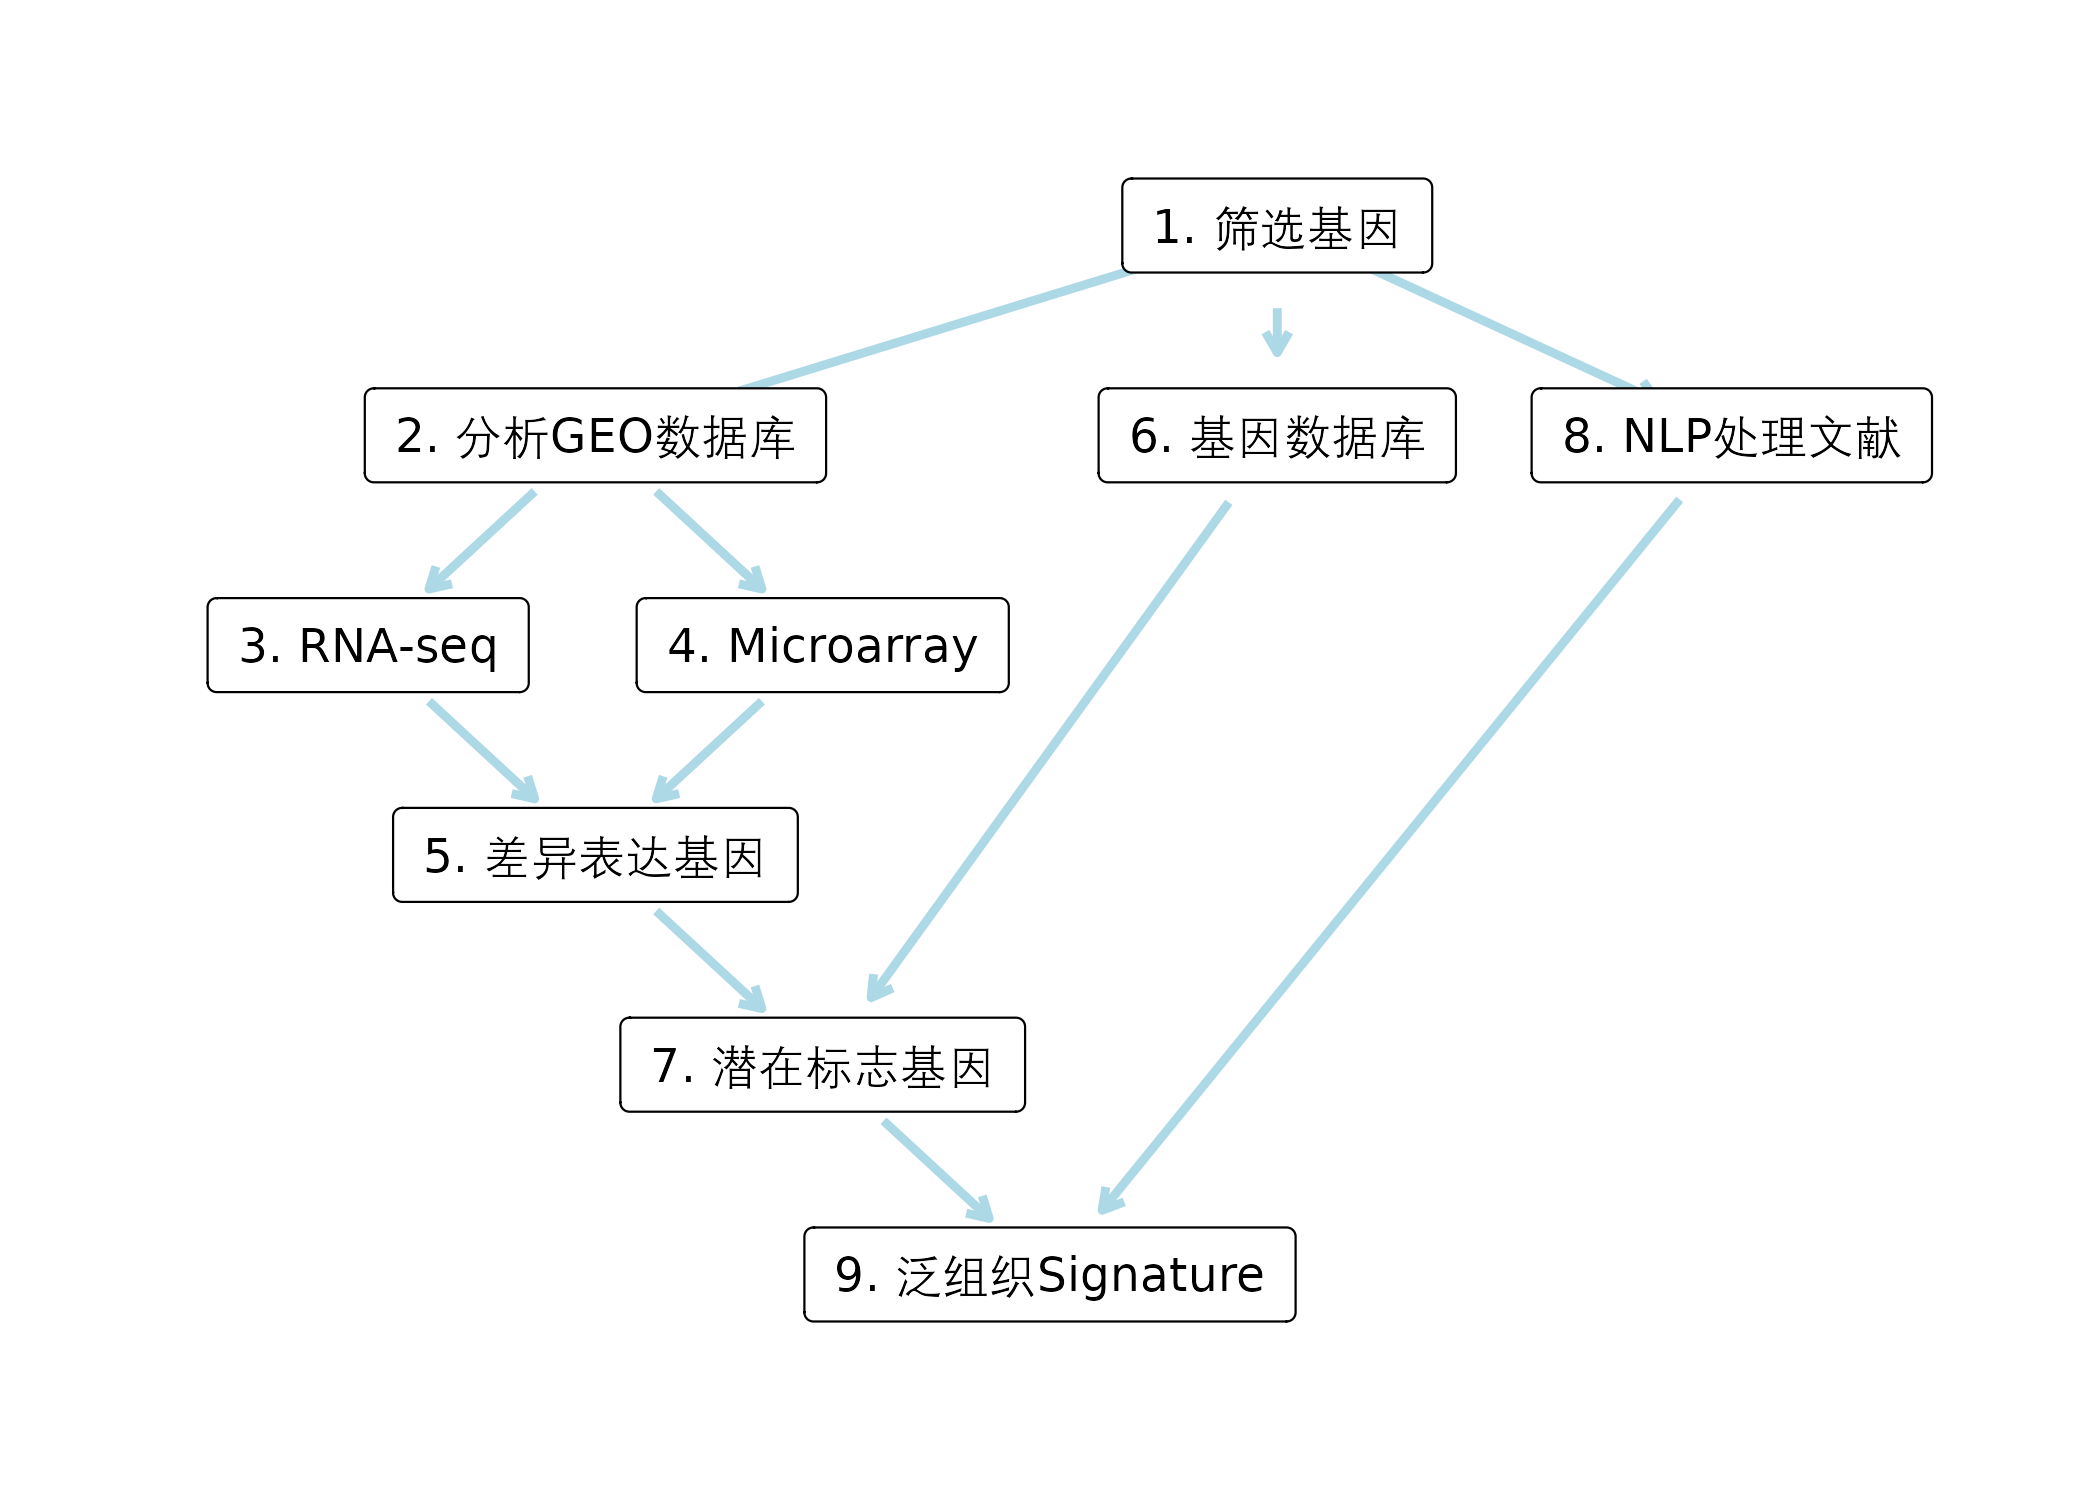
\includegraphics[width=24in]{thesis_fig/analysis_case} \caption{转录组分析案例流程示例}\label{fig:case1}
\makeatletter \egroup

\begin{enumerate}
\def\labelenumi{\arabic{enumi}.}
\tightlist
\item
  筛选基因结合:分析GEO数据库、筛选基因数据库、NLP处理文献。
\item
  分析GEO数据库,分析与AHR研究相关的疾病模型的数据集,根据差异性分析筛选基因。
\item
  RNA-seq,分析的GEO数据集的类型。
\item
  Microarray,分析的GEO数据集的类型。
\item
  差异表达基因,使用'limma'包分析得出,或者根据原研究者的研究数据筛选,根据'Q-value'、log\textsubscript{2}(FC)筛选。
\item
  检索转录因子靶向基因数据库(\url{https://tfbsdb.systemsbiology.net/})
\item
  将第5步筛选的差异表达基因与第6步检索到的基因取合集。
\item
  使用Java包(\url{https://julielab.de/Resources/JCoRe.html})处理报道有关AHR的文献。
\item
  将第7步和第8步取得的基因集取交集,获得泛组织AHR Signature基因
\end{enumerate}

\hypertarget{ux4ee3ux8c22ux7ec4ux5b66ux6848ux4f8b}{%
\subsection{代谢组学案例}\label{ux4ee3ux8c22ux7ec4ux5b66ux6848ux4f8b}}

为了示例编写的R包\href{https://github.com/Cao-lab-zcmu/MCnebula2}{MCnebula2}和其工作流的应用,在研究中曾重新分析MASSIVE中的代谢组数据集(\href{https://massive.ucsd.edu/ProteoSAFe/QueryMSV?id=MSV000083593}{MSV000083593})\textsuperscript{\protect\hyperlink{ref-2020s}{2}}。流程如下所述(Fig. \ref{fig:case2},代码和详细说明可见于\url{https://mcnebula.netlify.app/docs/workflow/serum_report_biocstyle}):

\bgroup \def\@captype{figure}
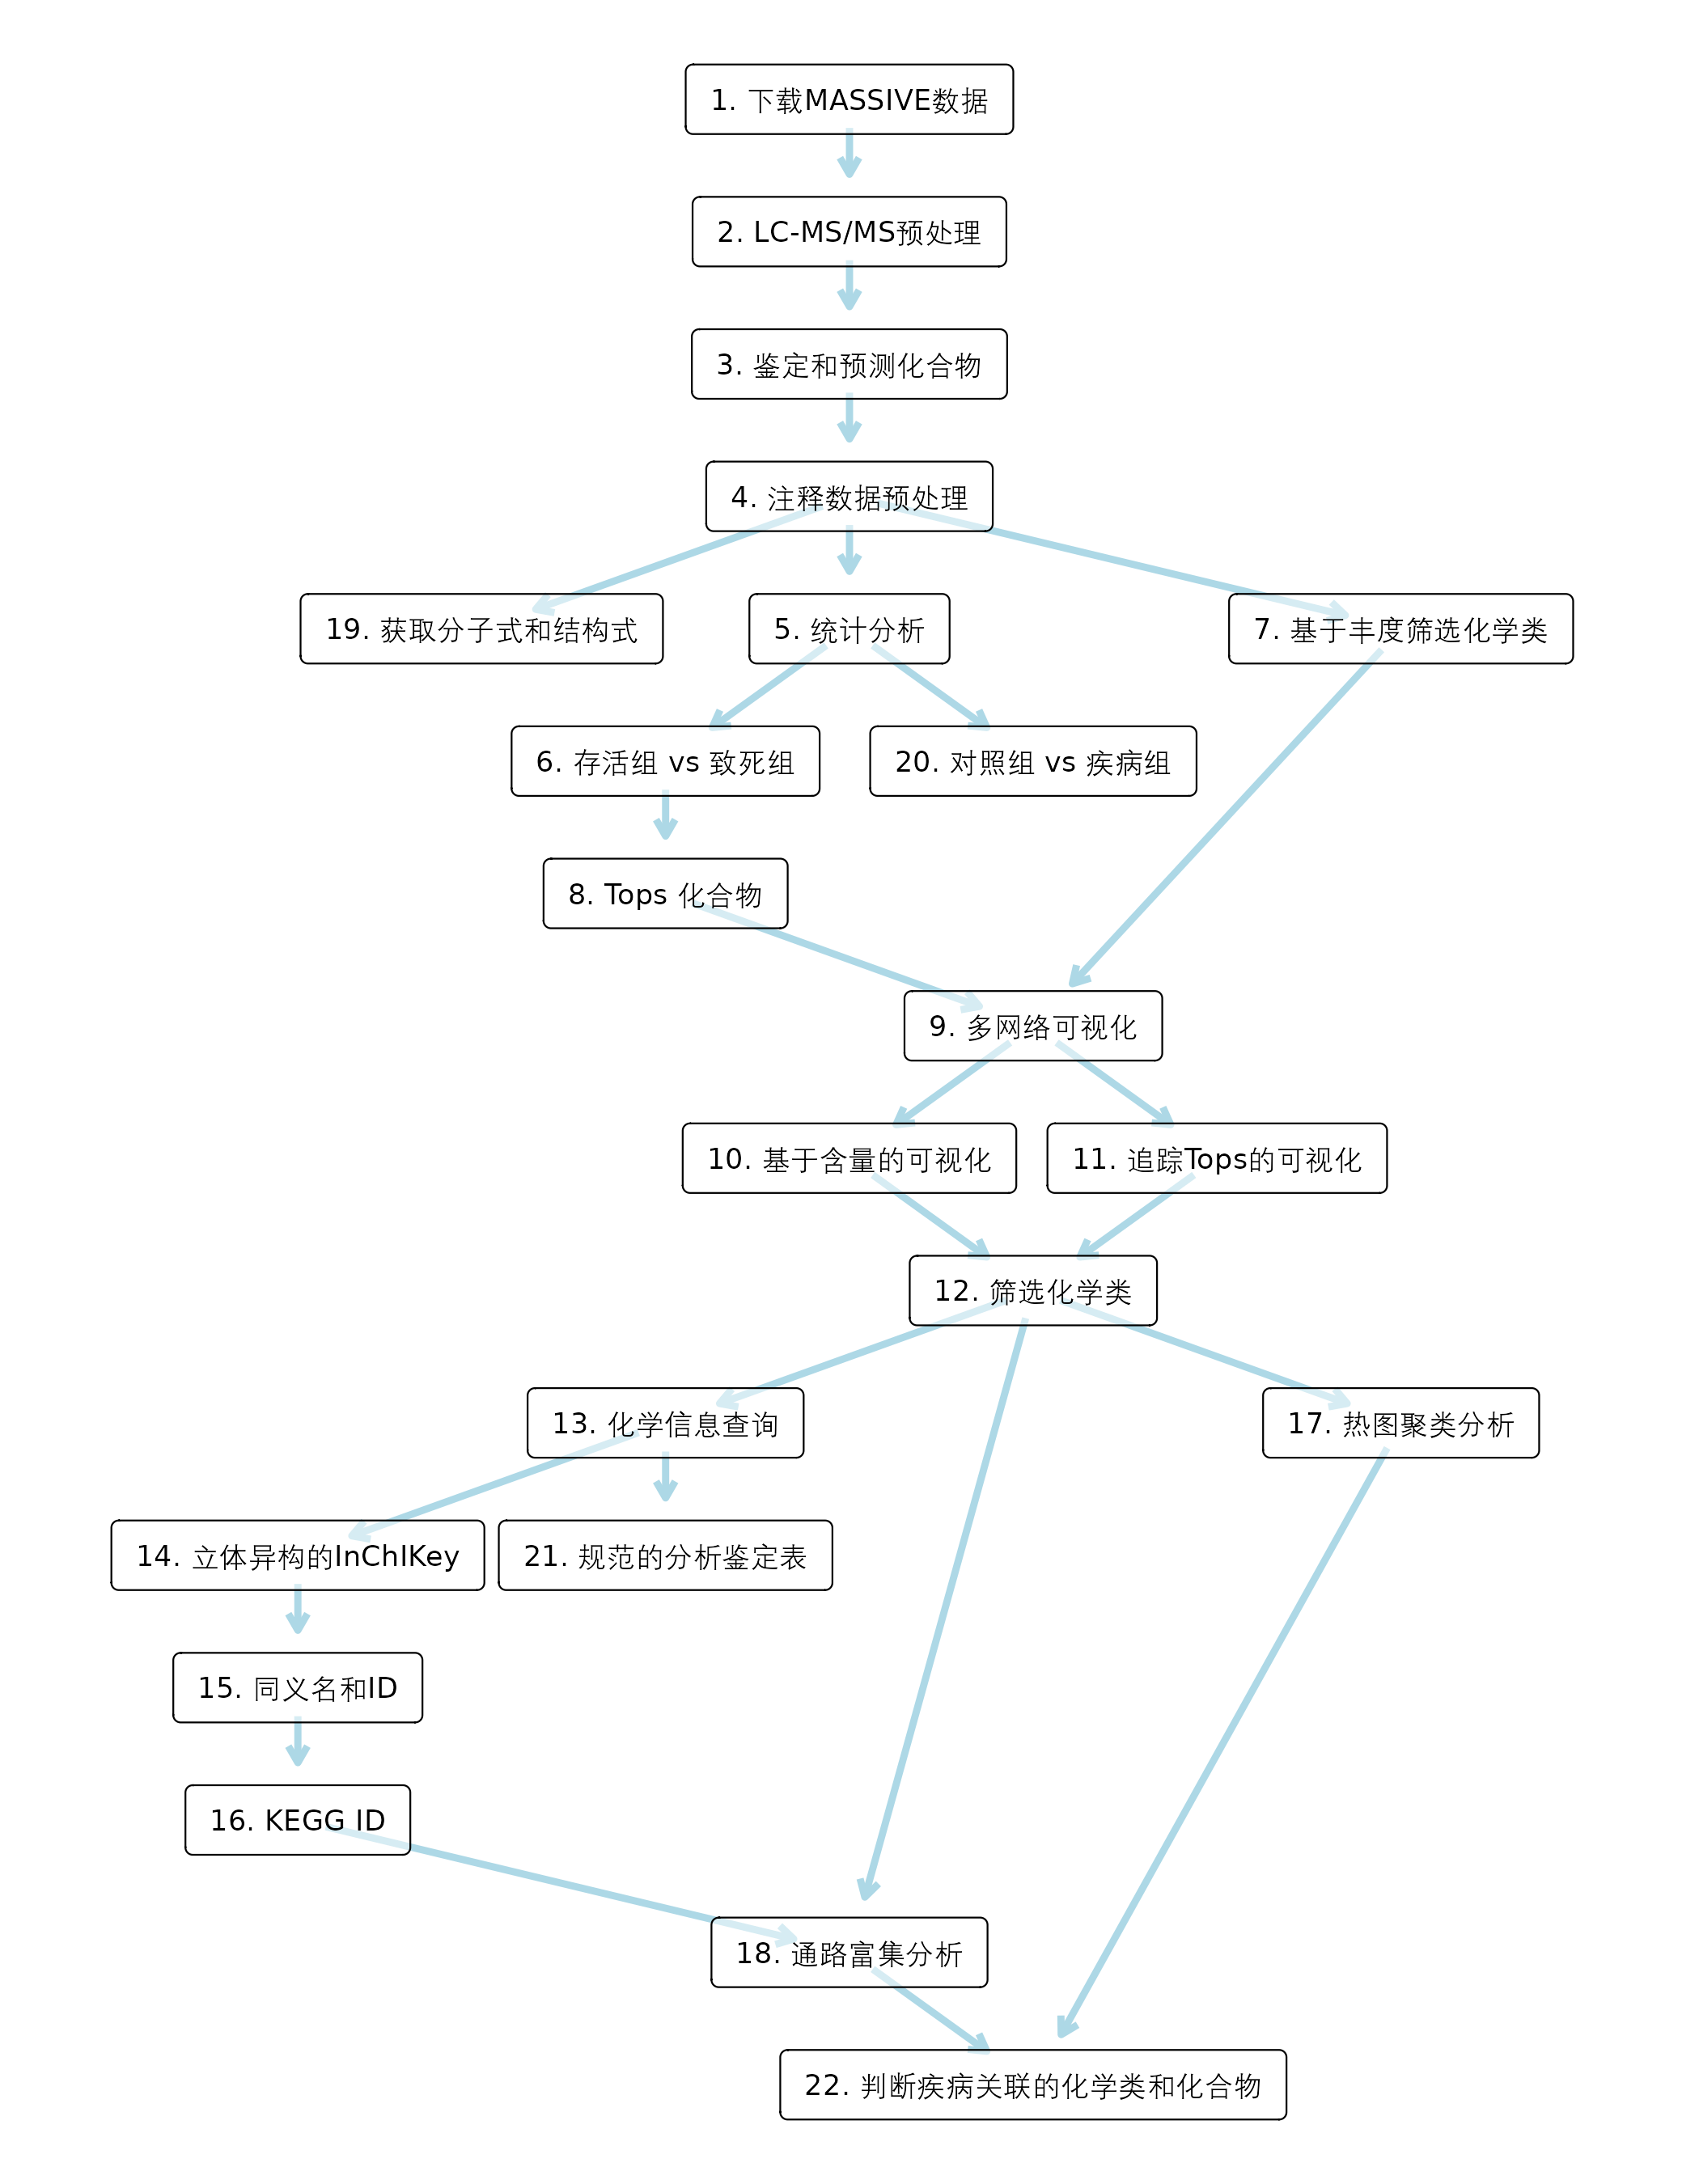
\includegraphics[width=25.14in]{thesis_fig/analysis_case2} \caption{代谢组分析案例流程示意}\label{fig:case2}
\makeatletter \egroup

\begin{enumerate}
\def\labelenumi{\arabic{enumi}.}
\tightlist
\item
  下载MASSIVE数据,即\href{https://massive.ucsd.edu/ProteoSAFe/QueryMSV?id=MSV000083593}{MSV000083593}
\item
  LC-MS/MS预处理,使用MZmine2进行峰检测和对齐等处理,并导出MS/MS信息的.mgf,定量信息的.csv。
\item
  鉴定和预测化合物,使用SIRIUS软件预测化合物的分子式、结构式、化学类等。
\item
  注释数据预处理,使用MCnebula2(以下分析均采用)R包整合并处理SIRIUS的注释数据。
\item
  统计分析,包括步骤6和步骤20,进行差异性分析。
\item
  存活组 vs 致死组,筛选两组间的差异代谢物。
\item
  基于丰度筛选化学类,MCnebula2提供的算法,根据化合物的化学类在整体数据集中的丰富程度筛选。
\item
  Tops 化合物,根据差异性分析的得分排名(例如Q-value),得到高排名的化合物。
\item
  多网络可视化,基于化学类将化合物聚类可视化为多个网络。
\item
  基于含量的可视化,将代谢物的含量变化水平呈现在网络图中。
\item
  追踪Tops的可视化,将Tops化合物标记在多网络图中,辅助筛选化学类。
\item
  筛选化学类,结合上述可视化筛选化学类。
\item
  化学信息查询,检索PubChem数据库,获取各类名称、ID和同义名信息(使用MCnebula2提供的函数)。
\item
  立体异构的InChIKey,质谱鉴定的程度达到分子骨架水平,可以以InChIKey2D表示,这一步在PubChem搜索所有InChIKey2D涵盖下的InChIKey(使用MCnebula2提供的函数)
\item
  同义名和ID,检索得到的化合物信息。
\item
  KEGG ID,代谢物的ID,从步骤15得到的ID信息的CID(PubChem CID)通过'MetaboAnalystR'包转化为KEGG ID。
\item
  热图聚类分析,根据步骤12筛选的化学类绘制聚类热图,判断该化学类与疾病的关联性。
\item
  通路富集分析,通过步骤16得到的KEGG ID进行富集分析,可以使用R的'FELLA'包,也能使用MetaboAnalyst网站提供的服务。
\item
  获取分子式和结构式,得到化合物的鉴定数据,用于注释网络图。
\item
  对照组 vs 疾病组,筛选两组间的差异代谢物。
\item
  规范的分析鉴定表,将鉴定数据和统计分析数据整合,得到可以用于论文发表的规范表格。
\item
  判断疾病关联的化学类和化合物,结合上述得出分析的结论,以备进一步验证。
\end{enumerate}

\hypertarget{geo-ux6570ux636eux5206ux6790}{%
\section{GEO 数据分析}\label{geo-ux6570ux636eux5206ux6790}}

\hypertarget{ux6570ux636eux96c6ux548cux76f8ux5173ux80ccux666f}{%
\subsection{数据集和相关背景}\label{ux6570ux636eux96c6ux548cux76f8ux5173ux80ccux666f}}

数据编号为:\href{https://www.ncbi.nlm.nih.gov/geo/query/acc.cgi?acc=GSE223325}{GSE223325}(Fig. \ref{fig:gse})。本数据集为较新的数据集,未见研究报道的记录。研究类风湿性关节炎单核细胞衍生巨噬细胞的促炎症和代谢功能。对极化的健康和类风湿关节炎单核细胞衍生的巨噬细胞进行了RNA测序。组别:

\begin{itemize}
\tightlist
\item
  对照组,24 hrs IL-4 (20ng/ml)。注:IL-4极化的巨噬细胞脂多糖(LPS)暴露后可建立一个高炎症基因表达程序\textsuperscript{\protect\hyperlink{ref-czimmerer_epigenetic_2022}{3}}。
\item
  模型组,24 hrs LPS (100ng/ml) and IFNg (20ng/ml)。注:由IFN-γ激活并由STAT1介导的前馈环路会放大细胞因子的信号,还会增强巨噬细胞对微生物诱导剂如Toll样受体(TLR)配体(例如LPS)的反应\textsuperscript{\protect\hyperlink{ref-hu_regulation_2008}{4},\protect\hyperlink{ref-chen_ifn-_2010}{5}}。
\end{itemize}

\bgroup \def\@captype{figure}
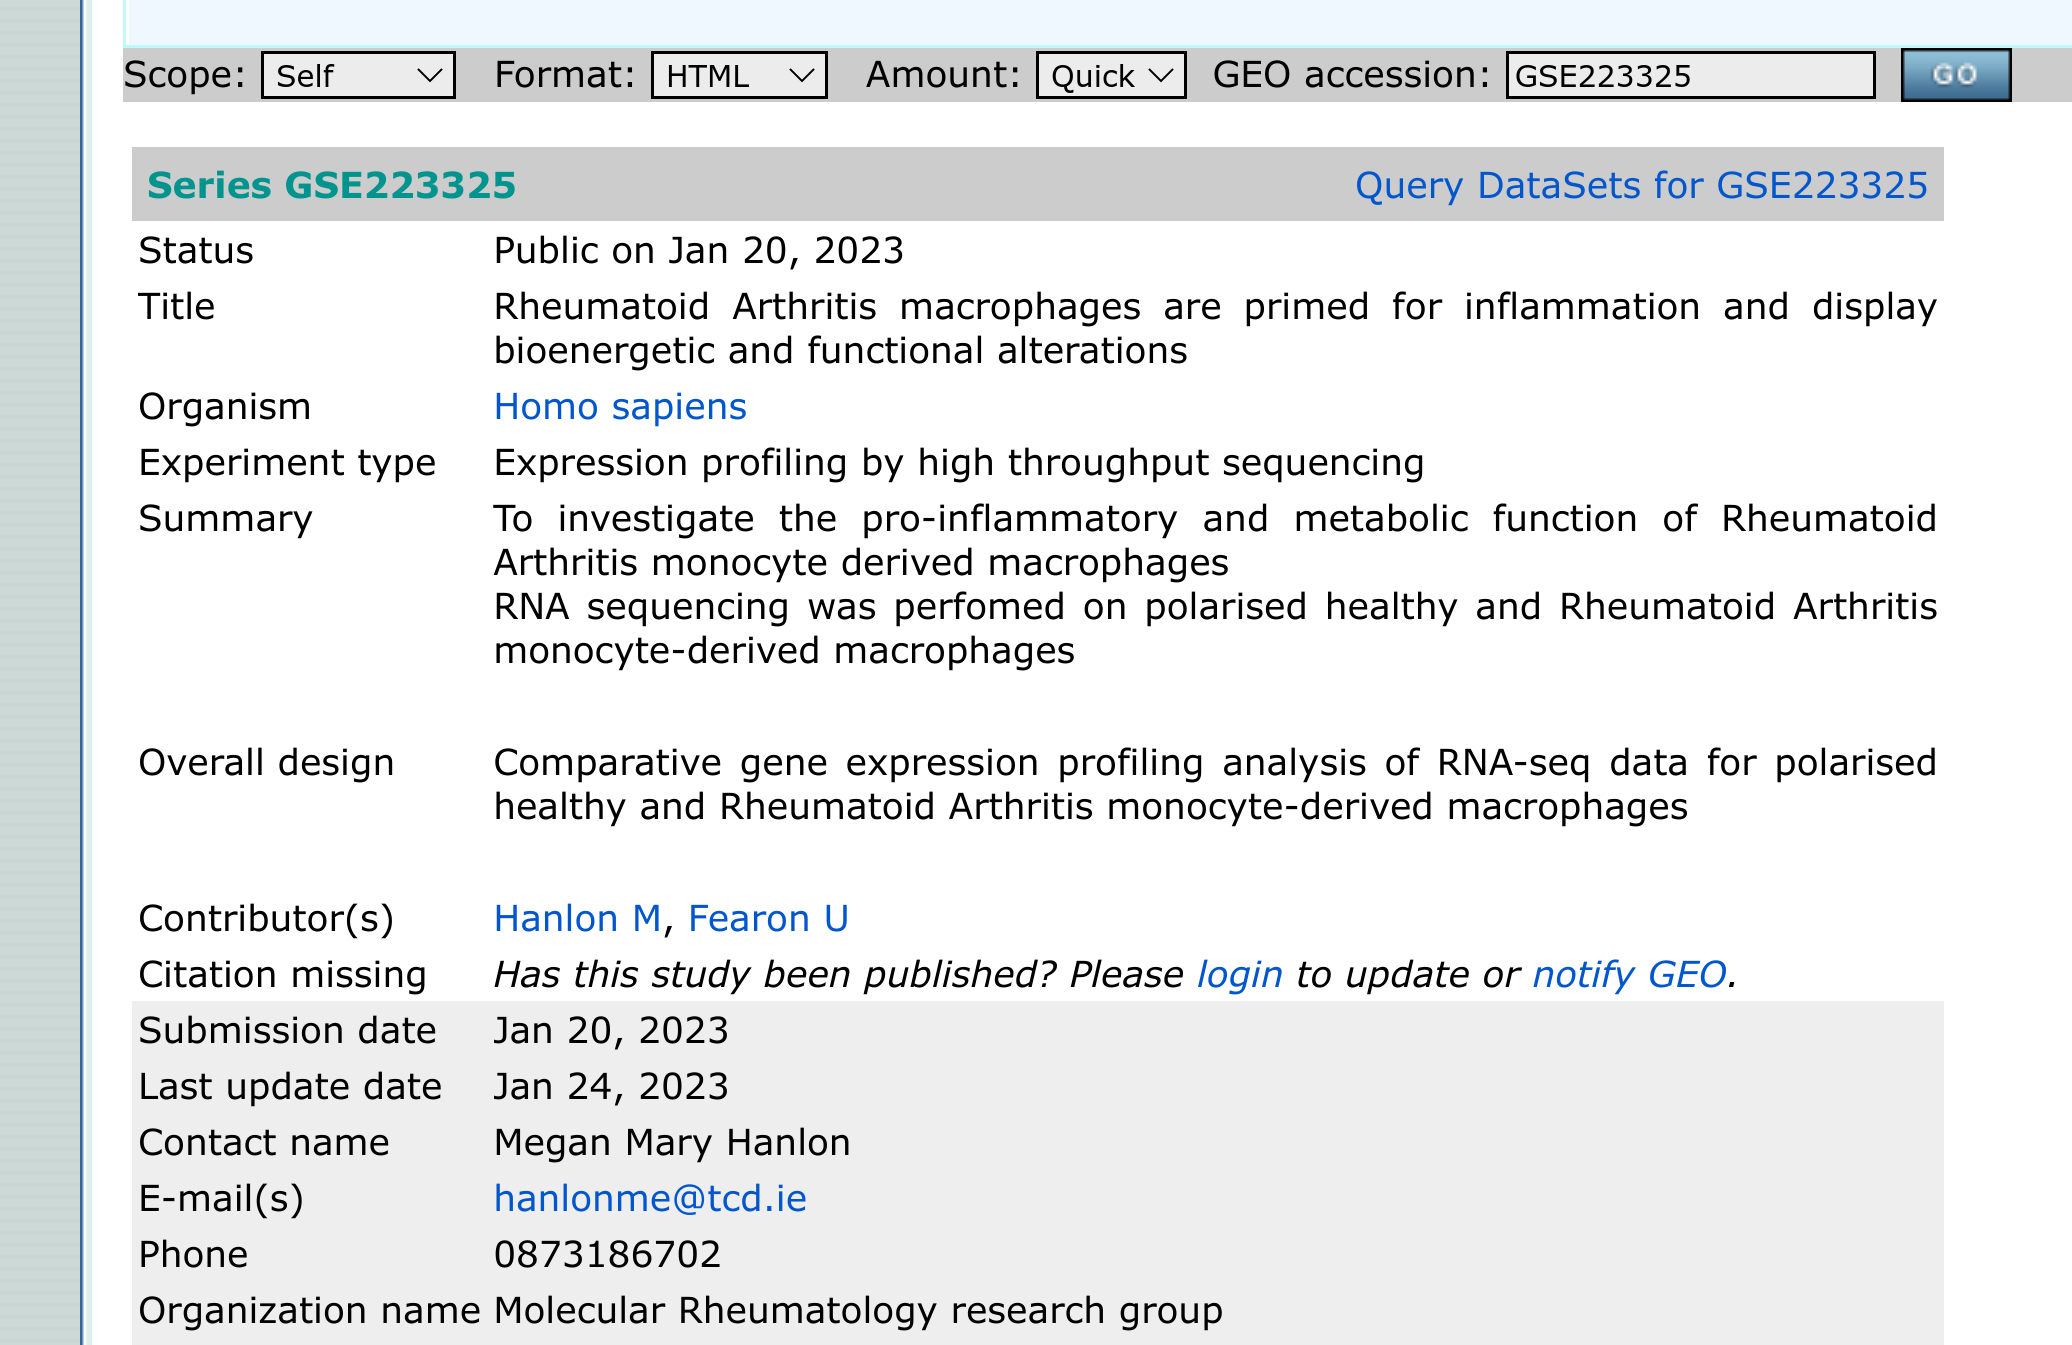
\includegraphics[width=13.89in]{thesis_fig/gse223325_capture} \caption{GSE223325数据集概览}\label{fig:gse}
\makeatletter \egroup

\hypertarget{ux8f6fux4ef6ux5de5ux5177ux8bedux8a00ux5305}{%
\subsection{软件、工具、语言包}\label{ux8f6fux4ef6ux5de5ux5177ux8bedux8a00ux5305}}

来源于CRAN的R包。

\begin{Shaded}
\begin{Highlighting}[]
\NormalTok{pkgs }\OtherTok{\textless{}{-}} \FunctionTok{c}\NormalTok{(}\StringTok{"dplyr"}\NormalTok{, }\StringTok{"data.table"}\NormalTok{, }\StringTok{"R.utils"}\NormalTok{,}
  \StringTok{"ggplot2"}\NormalTok{, }\StringTok{"BiocManager"}\NormalTok{, }\StringTok{"ggrepel"}\NormalTok{)}
\FunctionTok{lapply}\NormalTok{(pkgs,}
    \ControlFlowTok{function}\NormalTok{(pkg) \{}
      \ControlFlowTok{if}\NormalTok{ (}\SpecialCharTok{!}\FunctionTok{requireNamespace}\NormalTok{(pkg, }\AttributeTok{quietly =}\NormalTok{ T))}
        \FunctionTok{install.package}\NormalTok{(pkg)}
\NormalTok{    \})}
\end{Highlighting}
\end{Shaded}

来源于Bioconductor的包。

\begin{Shaded}
\begin{Highlighting}[]
\NormalTok{pkgs.bio }\OtherTok{\textless{}{-}} \FunctionTok{c}\NormalTok{(}\StringTok{"GEOquery"}\NormalTok{, }\StringTok{"edgeR"}\NormalTok{, }\StringTok{"limma"}\NormalTok{, }\StringTok{"pathview"}\NormalTok{,}
  \StringTok{"clusterProfiler"}\NormalTok{, }\StringTok{"biomaRt"}\NormalTok{)}
\FunctionTok{lapply}\NormalTok{(pkgs.bio,}
    \ControlFlowTok{function}\NormalTok{(pkg) \{}
      \ControlFlowTok{if}\NormalTok{ (}\SpecialCharTok{!}\FunctionTok{requireNamespace}\NormalTok{(pkg, }\AttributeTok{quietly =}\NormalTok{ T))}
\NormalTok{        BiocManager}\SpecialCharTok{::}\FunctionTok{install}\NormalTok{(pkg)}
\NormalTok{    \})}
\end{Highlighting}
\end{Shaded}

\hypertarget{ux5206ux6790ux6d41ux7a0b}{%
\subsection{分析流程}\label{ux5206ux6790ux6d41ux7a0b}}

本次分析的流程图见Fig. \ref{fig:GEOflow}。详情见\ref{steps}。

\bgroup \def\@captype{figure}
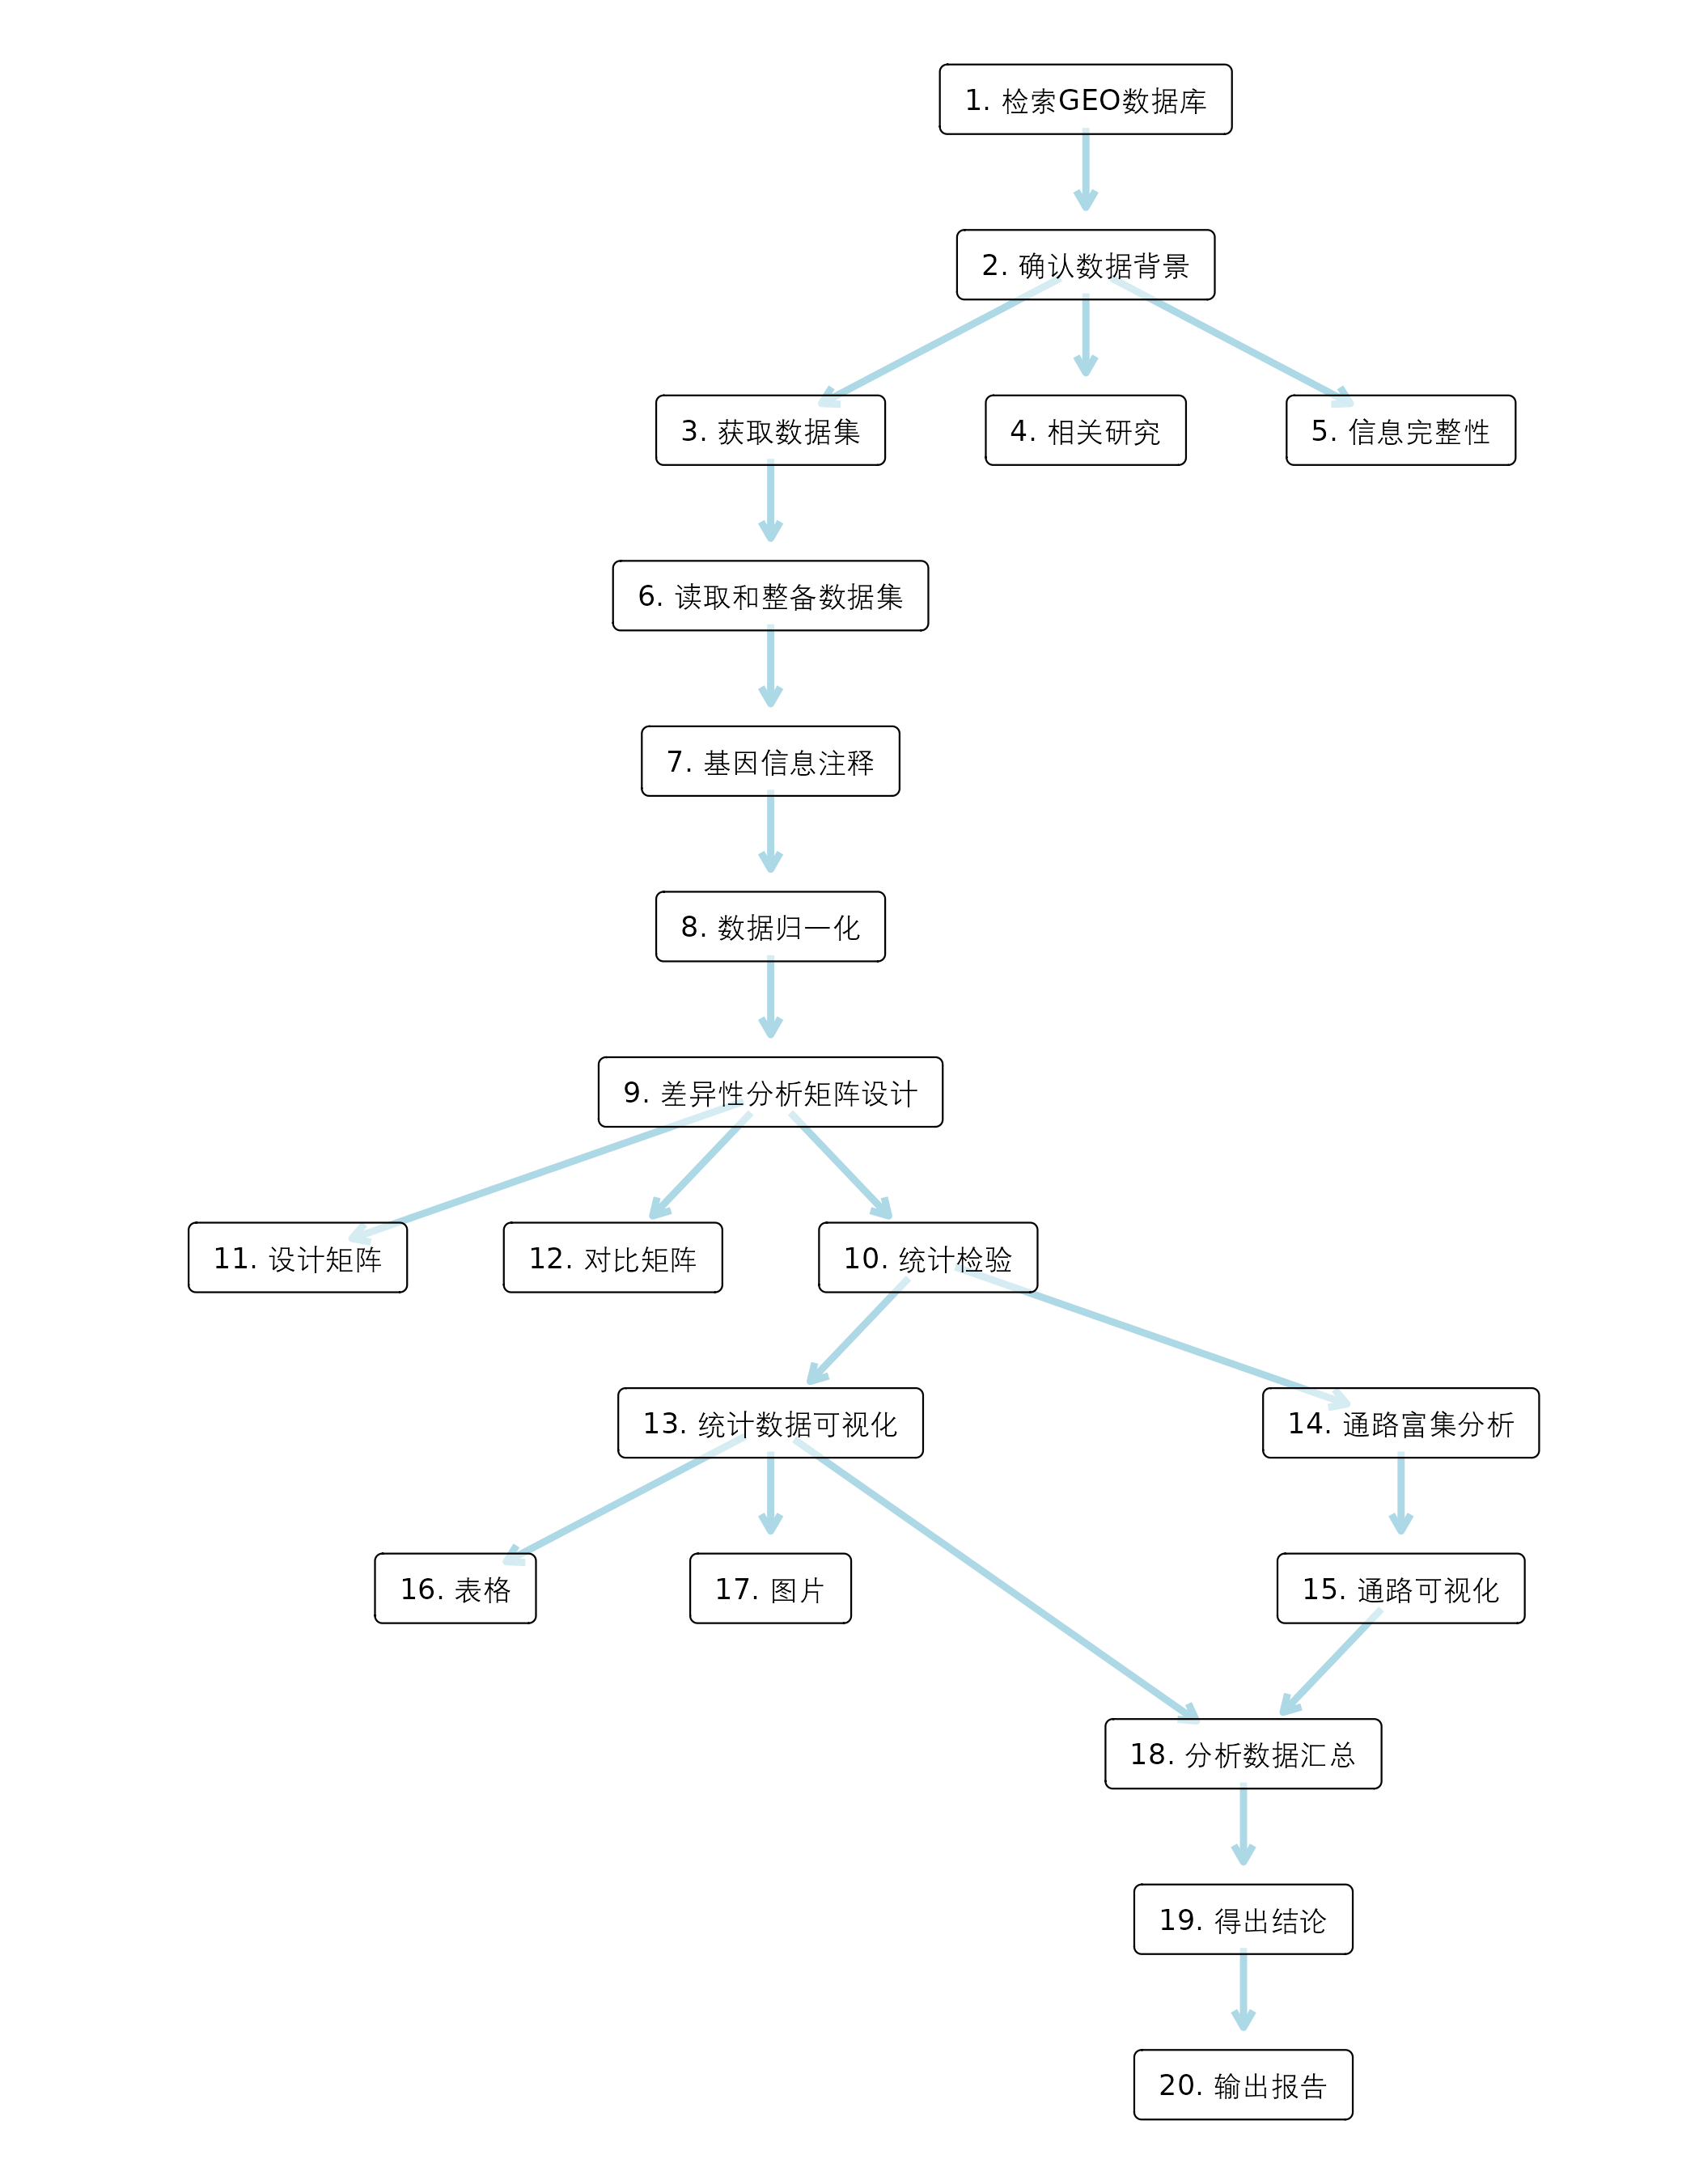
\includegraphics[width=23.22in]{thesis_fig/GEO_case} \caption{分析流程示意图}\label{fig:GEOflow}
\makeatletter \egroup

\hypertarget{steps}{%
\subsection{数据分析}\label{steps}}

\hypertarget{set-up}{%
\subsubsection{Set-up}\label{set-up}}

R的设定。只加载了\texttt{ggplot2}包,其他的包在使用时通过\texttt{::}调用。另外,个别函数用了自定义的函数,以免代码过于琐碎(对于关键性的步骤,没有使用自定义的函数)

\begin{Shaded}
\begin{Highlighting}[]
\FunctionTok{library}\NormalTok{(ggplot2)}
\DocumentationTok{\#\# The custom functions}
\NormalTok{bin }\OtherTok{\textless{}{-}}\NormalTok{ RCurl}\SpecialCharTok{::}\FunctionTok{getURLContent}\NormalTok{(}
  \FunctionTok{paste0}\NormalTok{(}\StringTok{"https://raw.githubusercontent.com/Cao{-}lab{-}zcmu/utils\_tool/"}\NormalTok{,}
    \StringTok{"master/R/tmp.ahr.R"}\NormalTok{)}
\NormalTok{)}
\FunctionTok{writeBin}\NormalTok{(bin, tmp }\OtherTok{\textless{}{-}} \FunctionTok{tempfile}\NormalTok{(}\AttributeTok{fileext =} \StringTok{".R"}\NormalTok{))}
\FunctionTok{source}\NormalTok{(tmp)}
\end{Highlighting}
\end{Shaded}

\hypertarget{ux83b7ux53d6ux6570ux636e}{%
\subsubsection{获取数据}\label{ux83b7ux53d6ux6570ux636e}}

使用R包\texttt{GEOquery}获取GEO数据。

\begin{Shaded}
\begin{Highlighting}[]
\NormalTok{gse }\OtherTok{\textless{}{-}} \StringTok{"GSE223325"}
\NormalTok{about }\OtherTok{\textless{}{-}}\NormalTok{ GEOquery}\SpecialCharTok{::}\FunctionTok{getGEO}\NormalTok{(gse)}
\end{Highlighting}
\end{Shaded}

查看数据已进行过的处理。

\begin{Shaded}
\begin{Highlighting}[]
\NormalTok{about[[}\DecValTok{1}\NormalTok{]]}\SpecialCharTok{$}\NormalTok{data\_processing}\FloatTok{.3}\NormalTok{[}\DecValTok{1}\NormalTok{]}
\end{Highlighting}
\end{Shaded}

\begin{verbatim}
## [1] "Supplementary files format and content: tab-delimited text files of TPM for each Sample"
\end{verbatim}

获取'GPL'的注释信息。

\begin{Shaded}
\begin{Highlighting}[]
\NormalTok{gpl }\OtherTok{\textless{}{-}}\NormalTok{ about[[}\DecValTok{1}\NormalTok{]]}\SpecialCharTok{@}\NormalTok{annotation}
\NormalTok{anno }\OtherTok{\textless{}{-}}\NormalTok{ GEOquery}\SpecialCharTok{::}\FunctionTok{getGEO}\NormalTok{(gpl)}
\NormalTok{org }\OtherTok{\textless{}{-}}\NormalTok{ anno}\SpecialCharTok{@}\NormalTok{header}\SpecialCharTok{$}\NormalTok{organism}
\end{Highlighting}
\end{Shaded}

将补充材料信息下载到本地(原作者处理过的包含TPM的矩阵数据)。

\begin{Shaded}
\begin{Highlighting}[]
\NormalTok{GEOquery}\SpecialCharTok{::}\FunctionTok{getGEOSuppFiles}\NormalTok{(gse)}
\NormalTok{utils}\SpecialCharTok{::}\FunctionTok{untar}\NormalTok{(}\FunctionTok{list.files}\NormalTok{(gse, }\AttributeTok{full.names =}\NormalTok{ T), }\AttributeTok{exdir =}\NormalTok{ gse)}
\FunctionTok{lapply}\NormalTok{(}\FunctionTok{list.files}\NormalTok{(gse, }\StringTok{"}\SpecialCharTok{\textbackslash{}\textbackslash{}}\StringTok{.gz$"}\NormalTok{, }\AttributeTok{full.names =}\NormalTok{ T), R.utils}\SpecialCharTok{::}\NormalTok{gunzip)}
\end{Highlighting}
\end{Shaded}

为样品信息创建元数据表格。

\begin{Shaded}
\begin{Highlighting}[]
\NormalTok{metadata }\OtherTok{\textless{}{-}} \FunctionTok{data.frame}\NormalTok{(}\AttributeTok{files =} \FunctionTok{list.files}\NormalTok{(gse, }\StringTok{"}\SpecialCharTok{\textbackslash{}\textbackslash{}}\StringTok{.txt$"}\NormalTok{, }\AttributeTok{full.names =}\NormalTok{ T)) }\SpecialCharTok{\%\textgreater{}\%} 
\NormalTok{  dplyr}\SpecialCharTok{::}\FunctionTok{mutate}\NormalTok{(}\AttributeTok{group =} \FunctionTok{ifelse}\NormalTok{(}\FunctionTok{grepl}\NormalTok{(}\StringTok{"M1}\SpecialCharTok{\textbackslash{}\textbackslash{}}\StringTok{.txt"}\NormalTok{, files), }\StringTok{"M1"}\NormalTok{, }\StringTok{"M2"}\NormalTok{),}
    \AttributeTok{group.anno =} \FunctionTok{ifelse}\NormalTok{(group }\SpecialCharTok{==} \StringTok{"M1"}\NormalTok{, }\StringTok{"LPC + IFN"}\NormalTok{, }\StringTok{"IL{-}4"}\NormalTok{),}
    \AttributeTok{sample =} \FunctionTok{gsub}\NormalTok{(}\StringTok{"\^{}.*/|}\SpecialCharTok{\textbackslash{}\textbackslash{}}\StringTok{.txt$"}\NormalTok{, }\StringTok{""}\NormalTok{, files)}
\NormalTok{  )}
\end{Highlighting}
\end{Shaded}

检查元数据表格,并查看矩阵数据状态。

\begin{Shaded}
\begin{Highlighting}[]
\NormalTok{metadata}
\end{Highlighting}
\end{Shaded}

\begin{verbatim}
##                             files group group.anno           sample
## 1  GSE223325/GSM6945621_RA1M1.txt    M1  LPC + IFN GSM6945621_RA1M1
## 2  GSE223325/GSM6945622_RA1M2.txt    M2       IL-4 GSM6945622_RA1M2
## 3  GSE223325/GSM6945623_RA2M1.txt    M1  LPC + IFN GSM6945623_RA2M1
## 4  GSE223325/GSM6945624_RA2M2.txt    M2       IL-4 GSM6945624_RA2M2
## 5  GSE223325/GSM6945625_RA3M1.txt    M1  LPC + IFN GSM6945625_RA3M1
## 6  GSE223325/GSM6945626_RA3M2.txt    M2       IL-4 GSM6945626_RA3M2
## 7  GSE223325/GSM6945627_RA4M1.txt    M1  LPC + IFN GSM6945627_RA4M1
## 8  GSE223325/GSM6945628_RA4M2.txt    M2       IL-4 GSM6945628_RA4M2
## 9  GSE223325/GSM6945629_RA5M1.txt    M1  LPC + IFN GSM6945629_RA5M1
## 10 GSE223325/GSM6945630_RA5M2.txt    M2       IL-4 GSM6945630_RA5M2
## 11 GSE223325/GSM6945631_RA6M1.txt    M1  LPC + IFN GSM6945631_RA6M1
## 12 GSE223325/GSM6945632_RA6M2.txt    M2       IL-4 GSM6945632_RA6M2
## 13 GSE223325/GSM6945633_RA7M1.txt    M1  LPC + IFN GSM6945633_RA7M1
## 14 GSE223325/GSM6945634_RA7M2.txt    M2       IL-4 GSM6945634_RA7M2
## 15 GSE223325/GSM6945635_RA8M1.txt    M1  LPC + IFN GSM6945635_RA8M1
## 16 GSE223325/GSM6945636_RA8M2.txt    M2       IL-4 GSM6945636_RA8M2
## 17 GSE223325/GSM6945637_RA9M1.txt    M1  LPC + IFN GSM6945637_RA9M1
## 18 GSE223325/GSM6945638_RA9M2.txt    M2       IL-4 GSM6945638_RA9M2
\end{verbatim}

\begin{Shaded}
\begin{Highlighting}[]
\NormalTok{tibble}\SpecialCharTok{::}\FunctionTok{as\_tibble}\NormalTok{(data.table}\SpecialCharTok{::}\FunctionTok{fread}\NormalTok{(}\StringTok{"./GSE223325/GSM6945621\_RA1M1.txt"}\NormalTok{))}
\end{Highlighting}
\end{Shaded}

\begin{verbatim}
## # A tibble: 60,504 x 4
##    V1                 V2    V3    V4
##    <chr>           <int> <int> <int>
##  1 ENSG00000223972     0     0     0
##  2 ENSG00000227232     0     0     0
##  3 ENSG00000278267     1     1     0
##  4 ENSG00000243485     0     0     0
##  5 ENSG00000274890     0     0     0
##  6 ENSG00000237613     0     0     0
##  7 ENSG00000268020     0     0     0
##  8 ENSG00000240361     0     0     0
##  9 ENSG00000186092     0     0     0
## 10 ENSG00000238009     3     2     1
## # ... with 60,494 more rows
\end{verbatim}

\hypertarget{diff}{%
\subsubsection{差异性分析}\label{diff}}

读取表达数据集。

\begin{Shaded}
\begin{Highlighting}[]
\NormalTok{dge.list }\OtherTok{\textless{}{-}}\NormalTok{ edgeR}\SpecialCharTok{::}\FunctionTok{readDGE}\NormalTok{(metadata}\SpecialCharTok{$}\NormalTok{files, }\AttributeTok{columns =} \FunctionTok{c}\NormalTok{(}\DecValTok{1}\NormalTok{, }\DecValTok{2}\NormalTok{))}
\NormalTok{dge.list }\OtherTok{\textless{}{-}} \FunctionTok{re.sample.group}\NormalTok{(dge.list, metadata)}
\end{Highlighting}
\end{Shaded}

使用R包'biomaRt'对基因信息进行注释。

\begin{Shaded}
\begin{Highlighting}[]
\NormalTok{ensembl }\OtherTok{\textless{}{-}}\NormalTok{ biomaRt}\SpecialCharTok{::}\FunctionTok{useEnsembl}\NormalTok{(}\AttributeTok{biomart =} \StringTok{"ensembl"}\NormalTok{, }\AttributeTok{dataset =} \StringTok{"hsapiens\_gene\_ensembl"}\NormalTok{)}
\NormalTok{attr }\OtherTok{\textless{}{-}} \FunctionTok{c}\NormalTok{(}\StringTok{"ensembl\_gene\_id"}\NormalTok{, }\StringTok{"hgnc\_symbol"}\NormalTok{, }\StringTok{"chromosome\_name"}\NormalTok{,}
        \StringTok{"start\_position"}\NormalTok{, }\StringTok{"end\_position"}\NormalTok{, }\StringTok{"description"}\NormalTok{)}
\NormalTok{gene.anno }\OtherTok{\textless{}{-}}\NormalTok{ biomaRt}\SpecialCharTok{::}\FunctionTok{getBM}\NormalTok{(attr, }\AttributeTok{mart =}\NormalTok{ ensembl)}
\NormalTok{gene.anno }\OtherTok{\textless{}{-}}\NormalTok{ tibble}\SpecialCharTok{::}\FunctionTok{as\_tibble}\NormalTok{(gene.anno)}
\NormalTok{dge.list }\OtherTok{\textless{}{-}} \FunctionTok{anno.into.list}\NormalTok{(dge.list, gene.anno, }\StringTok{"ensembl\_gene\_id"}\NormalTok{)}
\end{Highlighting}
\end{Shaded}

创建设计矩阵和对比矩阵\textsuperscript{\protect\hyperlink{ref-law_guide_2020}{6}}。

\begin{Shaded}
\begin{Highlighting}[]
\NormalTok{group. }\OtherTok{\textless{}{-}}\NormalTok{ dge.list}\SpecialCharTok{$}\NormalTok{samples}\SpecialCharTok{$}\NormalTok{group}
\NormalTok{design }\OtherTok{\textless{}{-}} \FunctionTok{model.matrix}\NormalTok{(}\SpecialCharTok{\textasciitilde{}} \DecValTok{0} \SpecialCharTok{+}\NormalTok{ group.)}
\NormalTok{contr.matrix }\OtherTok{\textless{}{-}}\NormalTok{ limma}\SpecialCharTok{::}\FunctionTok{makeContrasts}\NormalTok{(}
  \AttributeTok{M1\_vs\_M2 =}\NormalTok{ group.M1 }\SpecialCharTok{{-}}\NormalTok{ group.M2,}
  \AttributeTok{levels =}\NormalTok{ design}
\NormalTok{)}
\end{Highlighting}
\end{Shaded}

滤除低表达的基因信息。

\begin{Shaded}
\begin{Highlighting}[]
\NormalTok{keep.exprs }\OtherTok{\textless{}{-}}\NormalTok{ edgeR}\SpecialCharTok{::}\FunctionTok{filterByExpr}\NormalTok{(dge.list, }\AttributeTok{group =}\NormalTok{ group., }\AttributeTok{min.count =} \DecValTok{10}\NormalTok{)}
\NormalTok{dge.list }\OtherTok{\textless{}{-}}\NormalTok{ edgeR}\SpecialCharTok{::}\StringTok{\textasciigrave{}}\AttributeTok{[.DGEList}\StringTok{\textasciigrave{}}\NormalTok{(dge.list, keep.exprs, , }\AttributeTok{keep.lib.sizes =}\NormalTok{ F)}
\end{Highlighting}
\end{Shaded}

数据归一化。

\begin{Shaded}
\begin{Highlighting}[]
\NormalTok{dge.list }\OtherTok{\textless{}{-}}\NormalTok{ edgeR}\SpecialCharTok{::}\FunctionTok{calcNormFactors}\NormalTok{(dge.list, }\AttributeTok{method =} \StringTok{"TMM"}\NormalTok{)}
\NormalTok{dge.list }\OtherTok{\textless{}{-}}\NormalTok{ limma}\SpecialCharTok{::}\FunctionTok{voom}\NormalTok{(dge.list, design)}
\end{Highlighting}
\end{Shaded}

统计检验。

\begin{Shaded}
\begin{Highlighting}[]
\NormalTok{fit }\OtherTok{\textless{}{-}}\NormalTok{ limma}\SpecialCharTok{::}\FunctionTok{lmFit}\NormalTok{(dge.list, design)}
\NormalTok{fit.cont }\OtherTok{\textless{}{-}}\NormalTok{ limma}\SpecialCharTok{::}\FunctionTok{contrasts.fit}\NormalTok{(fit, }\AttributeTok{contrasts =}\NormalTok{ contr.matrix)}
\NormalTok{ebayes }\OtherTok{\textless{}{-}}\NormalTok{ limma}\SpecialCharTok{::}\FunctionTok{eBayes}\NormalTok{(fit.cont)}
\end{Highlighting}
\end{Shaded}

根据Q-value(FDR校正的P-value)和log\textsubscript{2}(FC)获取高排名的基因。

\begin{Shaded}
\begin{Highlighting}[]
\NormalTok{res }\OtherTok{\textless{}{-}}\NormalTok{ limma}\SpecialCharTok{::}\FunctionTok{topTable}\NormalTok{(ebayes, }\AttributeTok{coef =} \DecValTok{1}\NormalTok{, }\AttributeTok{number =} \ConstantTok{Inf}\NormalTok{)}
\NormalTok{res }\OtherTok{\textless{}{-}}\NormalTok{ tibble}\SpecialCharTok{::}\FunctionTok{as\_tibble}\NormalTok{(res)}
\NormalTok{res.tops }\OtherTok{\textless{}{-}}\NormalTok{ dplyr}\SpecialCharTok{::}\FunctionTok{filter}\NormalTok{(res, adj.P.Val }\SpecialCharTok{\textless{}}\NormalTok{ .}\DecValTok{05}\NormalTok{, }\FunctionTok{abs}\NormalTok{(logFC) }\SpecialCharTok{\textgreater{}} \DecValTok{1}\NormalTok{)}
\NormalTok{res.top30 }\OtherTok{\textless{}{-}} \FunctionTok{head}\NormalTok{(res.tops, }\AttributeTok{n =} \DecValTok{30}\NormalTok{)}
\end{Highlighting}
\end{Shaded}

检查结果。

\begin{Shaded}
\begin{Highlighting}[]
\NormalTok{res.top30}
\end{Highlighting}
\end{Shaded}

\begin{verbatim}
## # A tibble: 30 x 12
##    ensembl_gene_id hgnc_symbol  chromosome_name start_position end_position description       logFC
##    <chr>           <chr>        <chr>                    <int>        <int> <chr>             <dbl>
##  1 ENSG00000207508 "RNU6-1237P" 1                     40177843     40177949 RNA, U6 small nu~  3.02
##  2 ENSG00000154162 "CDH12"      5                     21750673     22853344 cadherin 12 [Sou~  4.45
##  3 ENSG00000235711 "ANKRD34C"   15                    79282722     79298239 ankyrin repeat d~  6.80
##  4 ENSG00000150045 "KLRF1"      12                     9827481      9845007 killer cell lect~  6.31
##  5 ENSG00000233996 "KDM3AP1"    2                    189486480    189487992 KDM3A pseudogene~  8.99
##  6 ENSG00000280344 ""           16                    51176066     51178898 TEC               -4.10
##  7 ENSG00000189367 "KIAA0408"   6                    127438406    127459389 KIAA0408 [Source~  3.23
##  8 ENSG00000120162 "MOB3B"      9                     27325209     27529814 MOB kinase activ~ 11.8 
##  9 ENSG00000234855 "SLIT1-AS1"  10                    97102756     97104355 SLIT1 antisense ~  2.42
## 10 ENSG00000137970 "RPL7P9"     1                     96678874     96679620 ribosomal protei~  7.83
## # ... with 20 more rows, and 5 more variables: AveExpr <dbl>, t <dbl>, P.Value <dbl>,
## #   adj.P.Val <dbl>, B <dbl>
\end{verbatim}

将结果可视化为火山图(Fig. \ref{fig:vol})。

\begin{Shaded}
\begin{Highlighting}[]
\NormalTok{data }\OtherTok{\textless{}{-}}\NormalTok{ dplyr}\SpecialCharTok{::}\FunctionTok{mutate}\NormalTok{(}
\NormalTok{  res.tops, }\AttributeTok{change =} \FunctionTok{ifelse}\NormalTok{(logFC }\SpecialCharTok{\textless{}} \SpecialCharTok{{-}}\DecValTok{1}\NormalTok{, }\StringTok{"down"}\NormalTok{,}
    \FunctionTok{ifelse}\NormalTok{(logFC }\SpecialCharTok{\textgreater{}} \DecValTok{1}\NormalTok{, }\StringTok{"up"}\NormalTok{, }\StringTok{"stable"}\NormalTok{))}
\NormalTok{)}
\NormalTok{p }\OtherTok{\textless{}{-}} \FunctionTok{ggplot}\NormalTok{(data, }\FunctionTok{aes}\NormalTok{(}\AttributeTok{x =}\NormalTok{ logFC, }\AttributeTok{y =} \SpecialCharTok{{-}}\FunctionTok{log10}\NormalTok{(adj.P.Val), }\AttributeTok{color =}\NormalTok{ change)) }\SpecialCharTok{+} 
        \FunctionTok{geom\_point}\NormalTok{(}\AttributeTok{alpha =} \FloatTok{0.8}\NormalTok{, }\AttributeTok{stroke =} \DecValTok{0}\NormalTok{, }\AttributeTok{size =} \DecValTok{3}\NormalTok{) }\SpecialCharTok{+} 
        \FunctionTok{scale\_color\_manual}\NormalTok{(}\AttributeTok{values =} \FunctionTok{c}\NormalTok{(}\StringTok{"down"} \OtherTok{=} \StringTok{"\#4DBBD5FF"}\NormalTok{,}
            \StringTok{"stable"} \OtherTok{=} \StringTok{"\#8491B4FF"}\NormalTok{,}
      \StringTok{"up"} \OtherTok{=} \StringTok{"\#DC0000FF"}\NormalTok{)) }\SpecialCharTok{+}
        \FunctionTok{ylim}\NormalTok{(}\DecValTok{1}\NormalTok{, }\FunctionTok{max}\NormalTok{(}\SpecialCharTok{{-}}\FunctionTok{log10}\NormalTok{(data}\SpecialCharTok{$}\NormalTok{adj.P.Val))) }\SpecialCharTok{+}
        \FunctionTok{geom\_hline}\NormalTok{(}\AttributeTok{yintercept =} \SpecialCharTok{{-}}\FunctionTok{log10}\NormalTok{(}\FloatTok{0.05}\NormalTok{), }\AttributeTok{linetype =} \DecValTok{4}\NormalTok{, }\AttributeTok{size =} \FloatTok{0.8}\NormalTok{) }\SpecialCharTok{+}
        \FunctionTok{geom\_vline}\NormalTok{(}\AttributeTok{xintercept =} \FunctionTok{c}\NormalTok{(}\SpecialCharTok{{-}}\DecValTok{1}\NormalTok{,}\DecValTok{1}\NormalTok{), }\AttributeTok{linetype =} \DecValTok{4}\NormalTok{, }\AttributeTok{size =} \FloatTok{0.8}\NormalTok{) }\SpecialCharTok{+} 
        \FunctionTok{labs}\NormalTok{(}\AttributeTok{x =} \StringTok{"log2(FC)"}\NormalTok{, }\AttributeTok{y =} \StringTok{"{-}log10(Q{-}value)"}\NormalTok{) }\SpecialCharTok{+} 
\NormalTok{    ggrepel}\SpecialCharTok{::}\FunctionTok{geom\_text\_repel}\NormalTok{(}
      \AttributeTok{data =}\NormalTok{ data[}\SpecialCharTok{{-}}\FunctionTok{log10}\NormalTok{(data}\SpecialCharTok{$}\NormalTok{adj.P.Val) }\SpecialCharTok{\textgreater{}} \FloatTok{7.5} \SpecialCharTok{\&} \FunctionTok{abs}\NormalTok{(data}\SpecialCharTok{$}\NormalTok{logFC) }\SpecialCharTok{\textgreater{}=} \FloatTok{7.5}\NormalTok{,],}
            \FunctionTok{aes}\NormalTok{(}\AttributeTok{label =}\NormalTok{ hgnc\_symbol),}
            \AttributeTok{size =} \DecValTok{3}\NormalTok{,}\AttributeTok{family=}\StringTok{"Times"}\NormalTok{) }\SpecialCharTok{+}
        \FunctionTok{theme}\NormalTok{(}\AttributeTok{text =} \FunctionTok{element\_text}\NormalTok{(}\AttributeTok{family =} \StringTok{"Times"}\NormalTok{))}
\FunctionTok{ggsave}\NormalTok{(p, }\AttributeTok{file =} \FunctionTok{paste0}\NormalTok{(}\StringTok{"volcano.png"}\NormalTok{), }\AttributeTok{height =} \FloatTok{5.5}\NormalTok{)}
\end{Highlighting}
\end{Shaded}

\bgroup \def\@captype{figure}
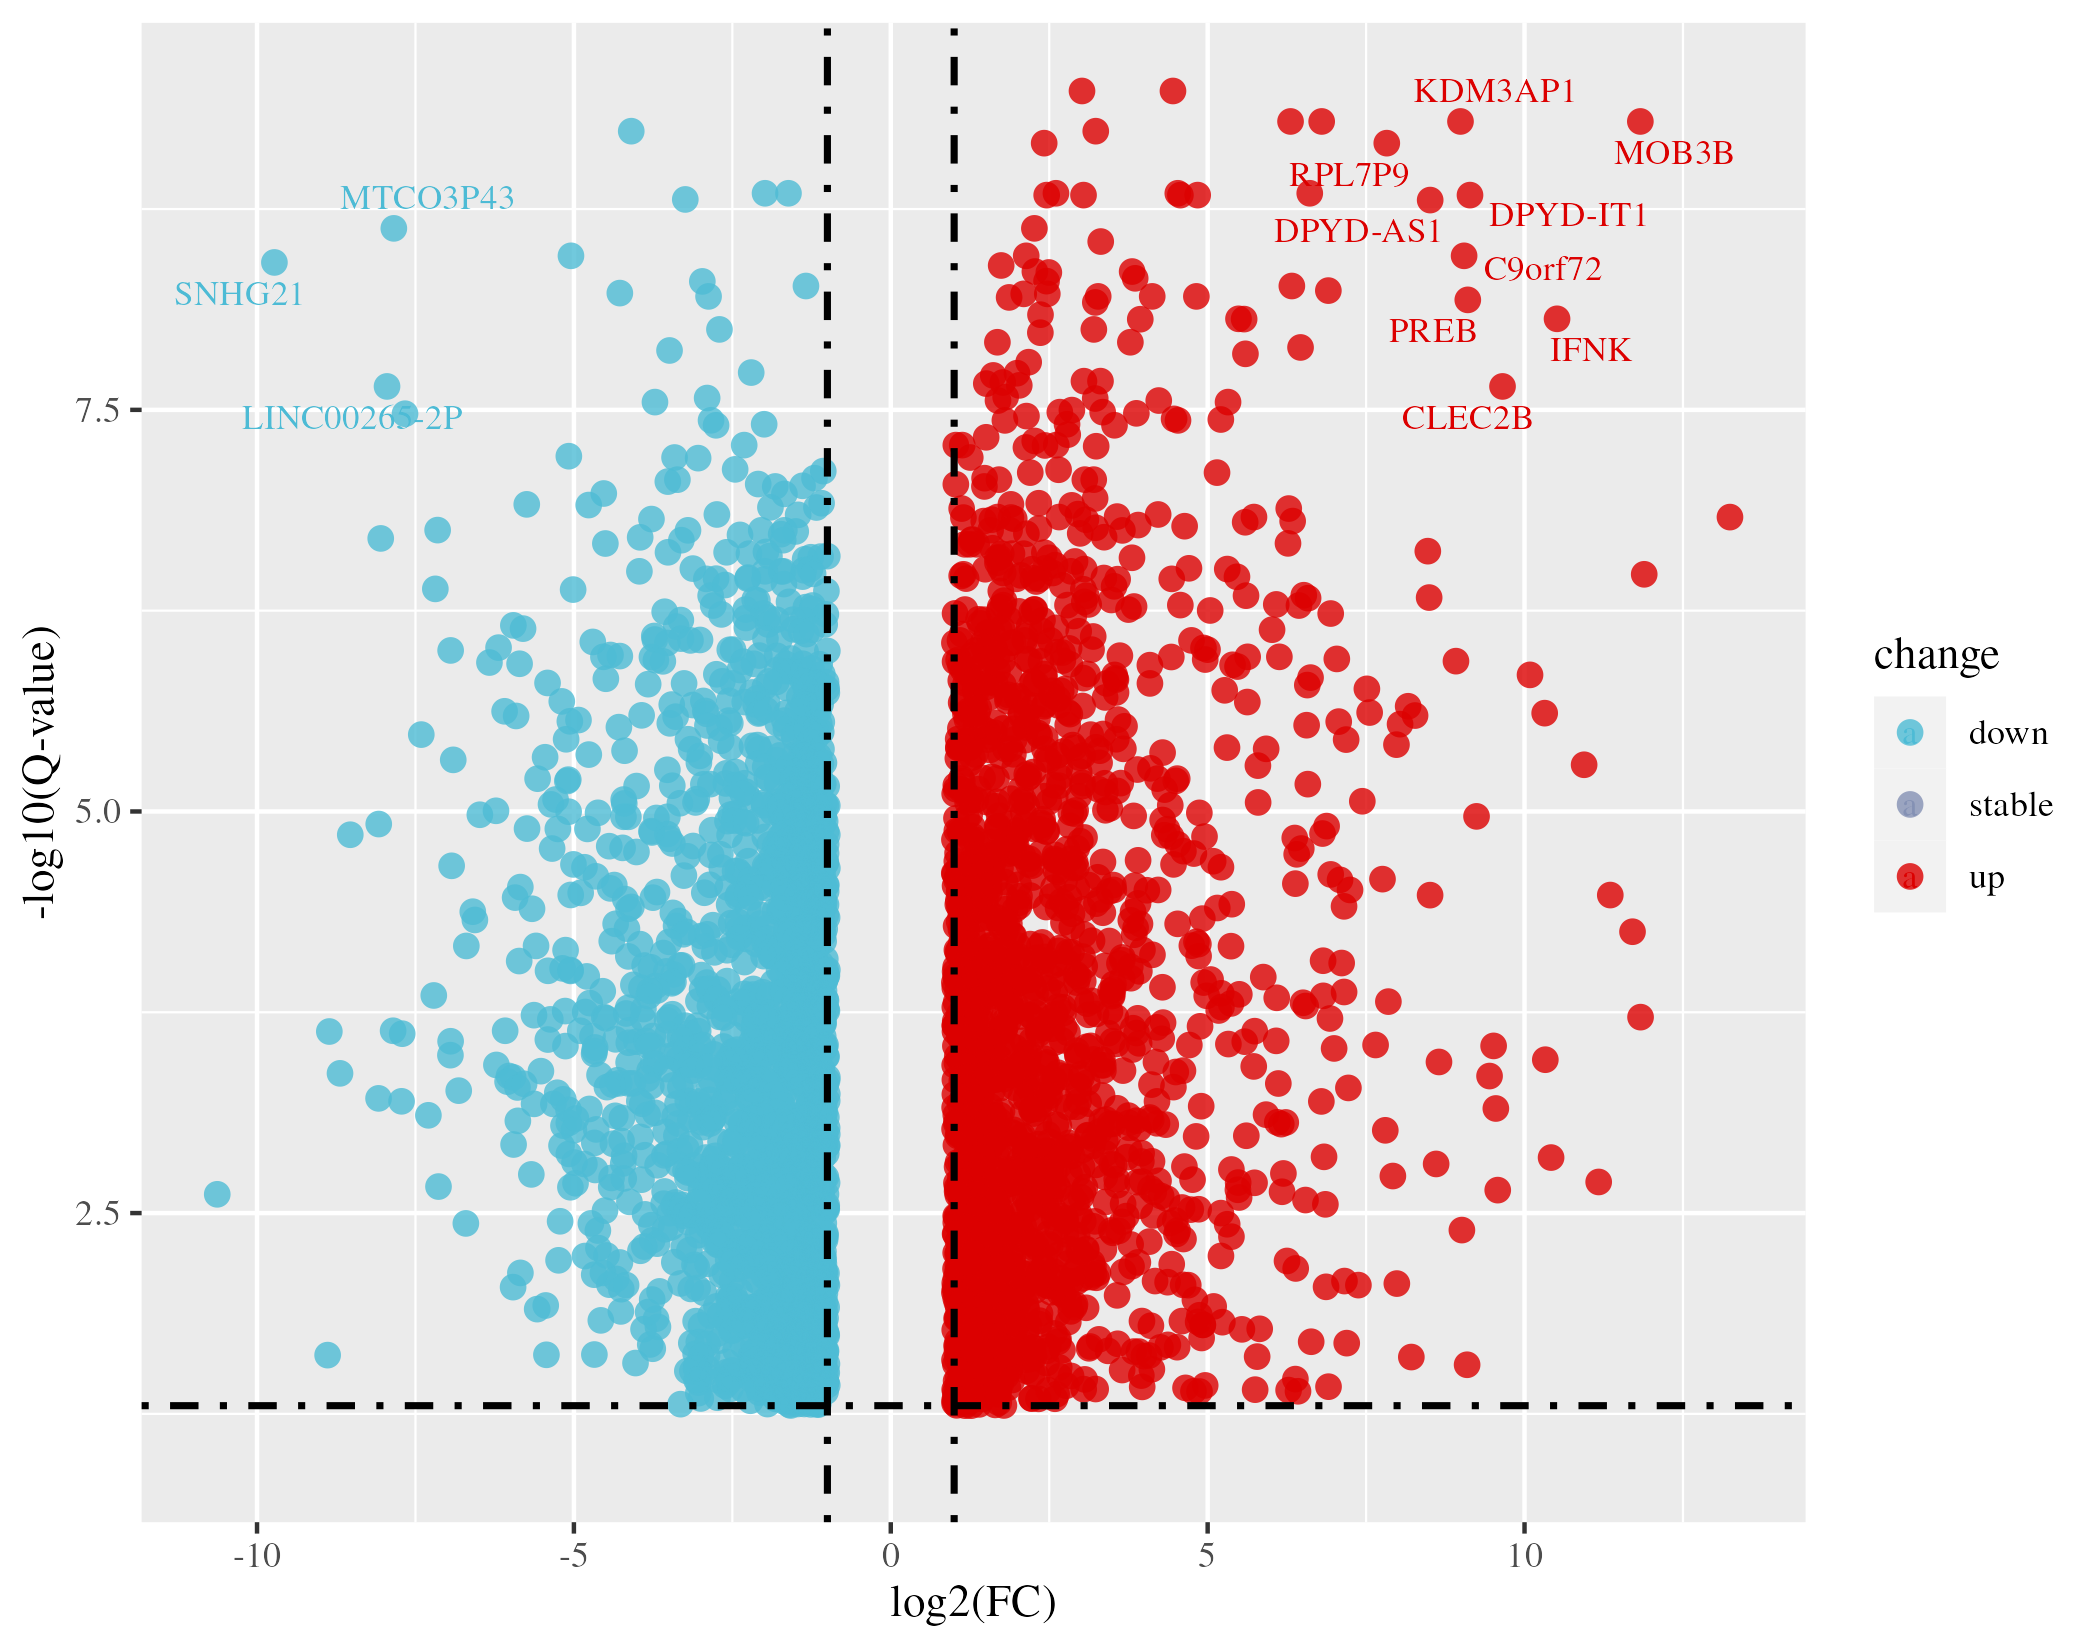
\includegraphics[width=28.22in]{thesis_fig/volcano} \caption{差异性分析结果的火山图可视化}\label{fig:vol}
\makeatletter \egroup

\hypertarget{ux529fux80fdux6ce8ux91ca}{%
\subsubsection{功能注释}\label{ux529fux80fdux6ce8ux91ca}}

在上一节\ref{diff}中,已经使用了\texttt{biomaRt}对基因进行了功能注释。Tab. \ref{tab:topAnno}显示Top 30的注释结果。

\hypertarget{ux901aux8defux5206ux6790}{%
\subsubsection{通路分析}\label{ux901aux8defux5206ux6790}}

\hypertarget{ux4f7fux7528clusterprofilerux901aux8defux5bccux96c6ux5206ux6790}{%
\paragraph{\texorpdfstring{使用\texttt{clusterProfiler}通路富集分析}{使用clusterProfiler通路富集分析}}\label{ux4f7fux7528clusterprofilerux901aux8defux5bccux96c6ux5206ux6790}}

使用R包\texttt{clusterProfiler}进行通路富集分析,在此之前,需要先将'ensembl ID'转化为'entrez ID'(一并展示在了Tab. \ref{tab:topAnno}中)。

\begin{Shaded}
\begin{Highlighting}[]
\NormalTok{ids }\OtherTok{\textless{}{-}}\NormalTok{ clusterProfiler}\SpecialCharTok{::}\FunctionTok{bitr}\NormalTok{(}
\NormalTok{  res.top30}\SpecialCharTok{$}\NormalTok{ensembl\_gene\_id, }\StringTok{"ENSEMBL"}\NormalTok{,}
  \StringTok{"ENTREZID"}\NormalTok{, }\StringTok{"org.Hs.eg.db"}\NormalTok{, F}
\NormalTok{)}
\NormalTok{ids }\OtherTok{\textless{}{-}}\NormalTok{ dplyr}\SpecialCharTok{::}\FunctionTok{distinct}\NormalTok{(ids, ENSEMBL, }\AttributeTok{.keep\_all =}\NormalTok{ T)}
\NormalTok{res.top30.ex }\OtherTok{\textless{}{-}}\NormalTok{ dplyr}\SpecialCharTok{::}\FunctionTok{mutate}\NormalTok{(res.top30, }\AttributeTok{entrezid =}\NormalTok{ ids[[}\DecValTok{2}\NormalTok{]]) }\SpecialCharTok{\%\textgreater{}\%} 
\NormalTok{  dplyr}\SpecialCharTok{::}\FunctionTok{filter}\NormalTok{(}\SpecialCharTok{!}\FunctionTok{is.na}\NormalTok{(entrezid))}
\end{Highlighting}
\end{Shaded}

\global\setlength{\Oldarrayrulewidth}{\arrayrulewidth}

\global\setlength{\Oldtabcolsep}{\tabcolsep}

\setlength{\tabcolsep}{0pt}

\renewcommand*{\arraystretch}{1.5}



\providecommand{\ascline}[3]{\noalign{\global\arrayrulewidth #1}\arrayrulecolor[HTML]{#2}\cline{#3}}

\begin{longtable}[c]{|p{1.20in}|p{1.20in}|p{1.20in}|p{2.40in}}

\caption{Top\ 30的基因功能注释(此处仅显示3列)}\label{tab:topAnno}\\

\ascline{1.5pt}{666666}{1-4}

\multicolumn{1}{>{\raggedright}m{\dimexpr 1.2in+0\tabcolsep}}{\textcolor[HTML]{000000}{\fontsize{10}{10}\selectfont{\global\setmainfont{Times New Roman}{Ensembl\ gene\ id}}}} & \multicolumn{1}{>{\raggedright}m{\dimexpr 1.2in+0\tabcolsep}}{\textcolor[HTML]{000000}{\fontsize{10}{10}\selectfont{\global\setmainfont{Times New Roman}{Hgnc\ symbol}}}} & \multicolumn{1}{>{\raggedright}m{\dimexpr 1.2in+0\tabcolsep}}{\textcolor[HTML]{000000}{\fontsize{10}{10}\selectfont{\global\setmainfont{Times New Roman}{Entrezid}}}} & \multicolumn{1}{>{\raggedright}m{\dimexpr 2.4in+0\tabcolsep}}{\textcolor[HTML]{000000}{\fontsize{10}{10}\selectfont{\global\setmainfont{Times New Roman}{Description}}}} \\

\ascline{1.5pt}{666666}{1-4}\endhead



\multicolumn{1}{>{\raggedright}p{\dimexpr 1.2in+0\tabcolsep}}{\textcolor[HTML]{000000}{\fontsize{10}{10}\selectfont{\global\setmainfont{Times New Roman}{ENSG00000207508}}}} & \multicolumn{1}{>{\raggedright}p{\dimexpr 1.2in+0\tabcolsep}}{\textcolor[HTML]{000000}{\fontsize{10}{10}\selectfont{\global\setmainfont{Times New Roman}{RNU6-1237P}}}} & \multicolumn{1}{>{\raggedright}p{\dimexpr 1.2in+0\tabcolsep}}{\textcolor[HTML]{000000}{\fontsize{10}{10}\selectfont{\global\setmainfont{Times New Roman}{106480651}}}} & \multicolumn{1}{>{\raggedright}p{\dimexpr 2.4in+0\tabcolsep}}{\textcolor[HTML]{000000}{\fontsize{10}{10}\selectfont{\global\setmainfont{Times New Roman}{RNA,\ U6\ small\ nuclear\ 1237,\ pseudogene\ [Source:HGNC\ Symbol;Acc:HGNC:48200]}}}} \\





\multicolumn{1}{>{\raggedright}p{\dimexpr 1.2in+0\tabcolsep}}{\textcolor[HTML]{000000}{\fontsize{10}{10}\selectfont{\global\setmainfont{Times New Roman}{ENSG00000154162}}}} & \multicolumn{1}{>{\raggedright}p{\dimexpr 1.2in+0\tabcolsep}}{\textcolor[HTML]{000000}{\fontsize{10}{10}\selectfont{\global\setmainfont{Times New Roman}{CDH12}}}} & \multicolumn{1}{>{\raggedright}p{\dimexpr 1.2in+0\tabcolsep}}{\textcolor[HTML]{000000}{\fontsize{10}{10}\selectfont{\global\setmainfont{Times New Roman}{1010}}}} & \multicolumn{1}{>{\raggedright}p{\dimexpr 2.4in+0\tabcolsep}}{\textcolor[HTML]{000000}{\fontsize{10}{10}\selectfont{\global\setmainfont{Times New Roman}{cadherin\ 12\ [Source:HGNC\ Symbol;Acc:HGNC:1751]}}}} \\





\multicolumn{1}{>{\raggedright}p{\dimexpr 1.2in+0\tabcolsep}}{\textcolor[HTML]{000000}{\fontsize{10}{10}\selectfont{\global\setmainfont{Times New Roman}{ENSG00000235711}}}} & \multicolumn{1}{>{\raggedright}p{\dimexpr 1.2in+0\tabcolsep}}{\textcolor[HTML]{000000}{\fontsize{10}{10}\selectfont{\global\setmainfont{Times New Roman}{ANKRD34C}}}} & \multicolumn{1}{>{\raggedright}p{\dimexpr 1.2in+0\tabcolsep}}{\textcolor[HTML]{000000}{\fontsize{10}{10}\selectfont{\global\setmainfont{Times New Roman}{390616}}}} & \multicolumn{1}{>{\raggedright}p{\dimexpr 2.4in+0\tabcolsep}}{\textcolor[HTML]{000000}{\fontsize{10}{10}\selectfont{\global\setmainfont{Times New Roman}{ankyrin\ repeat\ domain\ 34C\ [Source:HGNC\ Symbol;Acc:HGNC:33888]}}}} \\





\multicolumn{1}{>{\raggedright}p{\dimexpr 1.2in+0\tabcolsep}}{\textcolor[HTML]{000000}{\fontsize{10}{10}\selectfont{\global\setmainfont{Times New Roman}{ENSG00000150045}}}} & \multicolumn{1}{>{\raggedright}p{\dimexpr 1.2in+0\tabcolsep}}{\textcolor[HTML]{000000}{\fontsize{10}{10}\selectfont{\global\setmainfont{Times New Roman}{KLRF1}}}} & \multicolumn{1}{>{\raggedright}p{\dimexpr 1.2in+0\tabcolsep}}{\textcolor[HTML]{000000}{\fontsize{10}{10}\selectfont{\global\setmainfont{Times New Roman}{51348}}}} & \multicolumn{1}{>{\raggedright}p{\dimexpr 2.4in+0\tabcolsep}}{\textcolor[HTML]{000000}{\fontsize{10}{10}\selectfont{\global\setmainfont{Times New Roman}{killer\ cell\ lectin\ like\ receptor\ F1\ [Source:HGNC\ Symbol;Acc:HGNC:13342]}}}} \\





\multicolumn{1}{>{\raggedright}p{\dimexpr 1.2in+0\tabcolsep}}{\textcolor[HTML]{000000}{\fontsize{10}{10}\selectfont{\global\setmainfont{Times New Roman}{ENSG00000189367}}}} & \multicolumn{1}{>{\raggedright}p{\dimexpr 1.2in+0\tabcolsep}}{\textcolor[HTML]{000000}{\fontsize{10}{10}\selectfont{\global\setmainfont{Times New Roman}{KIAA0408}}}} & \multicolumn{1}{>{\raggedright}p{\dimexpr 1.2in+0\tabcolsep}}{\textcolor[HTML]{000000}{\fontsize{10}{10}\selectfont{\global\setmainfont{Times New Roman}{9729}}}} & \multicolumn{1}{>{\raggedright}p{\dimexpr 2.4in+0\tabcolsep}}{\textcolor[HTML]{000000}{\fontsize{10}{10}\selectfont{\global\setmainfont{Times New Roman}{KIAA0408\ [Source:HGNC\ Symbol;Acc:HGNC:21636]}}}} \\





\multicolumn{1}{>{\raggedright}p{\dimexpr 1.2in+0\tabcolsep}}{\textcolor[HTML]{000000}{\fontsize{10}{10}\selectfont{\global\setmainfont{Times New Roman}{ENSG00000120162}}}} & \multicolumn{1}{>{\raggedright}p{\dimexpr 1.2in+0\tabcolsep}}{\textcolor[HTML]{000000}{\fontsize{10}{10}\selectfont{\global\setmainfont{Times New Roman}{MOB3B}}}} & \multicolumn{1}{>{\raggedright}p{\dimexpr 1.2in+0\tabcolsep}}{\textcolor[HTML]{000000}{\fontsize{10}{10}\selectfont{\global\setmainfont{Times New Roman}{79817}}}} & \multicolumn{1}{>{\raggedright}p{\dimexpr 2.4in+0\tabcolsep}}{\textcolor[HTML]{000000}{\fontsize{10}{10}\selectfont{\global\setmainfont{Times New Roman}{MOB\ kinase\ activator\ 3B\ [Source:HGNC\ Symbol;Acc:HGNC:23825]}}}} \\





\multicolumn{1}{>{\raggedright}p{\dimexpr 1.2in+0\tabcolsep}}{\textcolor[HTML]{000000}{\fontsize{10}{10}\selectfont{\global\setmainfont{Times New Roman}{ENSG00000234855}}}} & \multicolumn{1}{>{\raggedright}p{\dimexpr 1.2in+0\tabcolsep}}{\textcolor[HTML]{000000}{\fontsize{10}{10}\selectfont{\global\setmainfont{Times New Roman}{SLIT1-AS1}}}} & \multicolumn{1}{>{\raggedright}p{\dimexpr 1.2in+0\tabcolsep}}{\textcolor[HTML]{000000}{\fontsize{10}{10}\selectfont{\global\setmainfont{Times New Roman}{100505540}}}} & \multicolumn{1}{>{\raggedright}p{\dimexpr 2.4in+0\tabcolsep}}{\textcolor[HTML]{000000}{\fontsize{10}{10}\selectfont{\global\setmainfont{Times New Roman}{SLIT1\ antisense\ RNA\ 1\ [Source:HGNC\ Symbol;Acc:HGNC:51198]}}}} \\





\multicolumn{1}{>{\raggedright}p{\dimexpr 1.2in+0\tabcolsep}}{\textcolor[HTML]{000000}{\fontsize{10}{10}\selectfont{\global\setmainfont{Times New Roman}{ENSG00000137970}}}} & \multicolumn{1}{>{\raggedright}p{\dimexpr 1.2in+0\tabcolsep}}{\textcolor[HTML]{000000}{\fontsize{10}{10}\selectfont{\global\setmainfont{Times New Roman}{RPL7P9}}}} & \multicolumn{1}{>{\raggedright}p{\dimexpr 1.2in+0\tabcolsep}}{\textcolor[HTML]{000000}{\fontsize{10}{10}\selectfont{\global\setmainfont{Times New Roman}{653702}}}} & \multicolumn{1}{>{\raggedright}p{\dimexpr 2.4in+0\tabcolsep}}{\textcolor[HTML]{000000}{\fontsize{10}{10}\selectfont{\global\setmainfont{Times New Roman}{ribosomal\ protein\ L7\ pseudogene\ 9\ [Source:HGNC\ Symbol;Acc:HGNC:37028]}}}} \\





\multicolumn{1}{>{\raggedright}p{\dimexpr 1.2in+0\tabcolsep}}{\textcolor[HTML]{000000}{\fontsize{10}{10}\selectfont{\global\setmainfont{Times New Roman}{ENSG00000251223}}}} & \multicolumn{1}{>{\raggedright}p{\dimexpr 1.2in+0\tabcolsep}}{\textcolor[HTML]{000000}{\fontsize{10}{10}\selectfont{\global\setmainfont{Times New Roman}{MTCO1P9}}}} & \multicolumn{1}{>{\raggedright}p{\dimexpr 1.2in+0\tabcolsep}}{\textcolor[HTML]{000000}{\fontsize{10}{10}\selectfont{\global\setmainfont{Times New Roman}{107075139}}}} & \multicolumn{1}{>{\raggedright}p{\dimexpr 2.4in+0\tabcolsep}}{\textcolor[HTML]{000000}{\fontsize{10}{10}\selectfont{\global\setmainfont{Times New Roman}{MT-CO1\ pseudogene\ 9\ [Source:HGNC\ Symbol;Acc:HGNC:52011]}}}} \\





\multicolumn{1}{>{\raggedright}p{\dimexpr 1.2in+0\tabcolsep}}{\textcolor[HTML]{000000}{\fontsize{10}{10}\selectfont{\global\setmainfont{Times New Roman}{ENSG00000242423}}}} & \multicolumn{1}{>{\raggedright}p{\dimexpr 1.2in+0\tabcolsep}}{\textcolor[HTML]{000000}{\fontsize{10}{10}\selectfont{\global\setmainfont{Times New Roman}{RPL12P36}}}} & \multicolumn{1}{>{\raggedright}p{\dimexpr 1.2in+0\tabcolsep}}{\textcolor[HTML]{000000}{\fontsize{10}{10}\selectfont{\global\setmainfont{Times New Roman}{100271408}}}} & \multicolumn{1}{>{\raggedright}p{\dimexpr 2.4in+0\tabcolsep}}{\textcolor[HTML]{000000}{\fontsize{10}{10}\selectfont{\global\setmainfont{Times New Roman}{ribosomal\ protein\ L12\ pseudogene\ 36\ [Source:HGNC\ Symbol;Acc:HGNC:36598]}}}} \\





\multicolumn{1}{>{\raggedright}p{\dimexpr 1.2in+0\tabcolsep}}{\textcolor[HTML]{000000}{\fontsize{10}{10}\selectfont{\global\setmainfont{Times New Roman}{ENSG00000265420}}}} & \multicolumn{1}{>{\raggedright}p{\dimexpr 1.2in+0\tabcolsep}}{\textcolor[HTML]{000000}{\fontsize{10}{10}\selectfont{\global\setmainfont{Times New Roman}{MIR4779}}}} & \multicolumn{1}{>{\raggedright}p{\dimexpr 1.2in+0\tabcolsep}}{\textcolor[HTML]{000000}{\fontsize{10}{10}\selectfont{\global\setmainfont{Times New Roman}{100616159}}}} & \multicolumn{1}{>{\raggedright}p{\dimexpr 2.4in+0\tabcolsep}}{\textcolor[HTML]{000000}{\fontsize{10}{10}\selectfont{\global\setmainfont{Times New Roman}{microRNA\ 4779\ [Source:HGNC\ Symbol;Acc:HGNC:41747]}}}} \\





\multicolumn{1}{>{\raggedright}p{\dimexpr 1.2in+0\tabcolsep}}{\textcolor[HTML]{000000}{\fontsize{10}{10}\selectfont{\global\setmainfont{Times New Roman}{ENSG00000117569}}}} & \multicolumn{1}{>{\raggedright}p{\dimexpr 1.2in+0\tabcolsep}}{\textcolor[HTML]{000000}{\fontsize{10}{10}\selectfont{\global\setmainfont{Times New Roman}{PTBP2}}}} & \multicolumn{1}{>{\raggedright}p{\dimexpr 1.2in+0\tabcolsep}}{\textcolor[HTML]{000000}{\fontsize{10}{10}\selectfont{\global\setmainfont{Times New Roman}{58155}}}} & \multicolumn{1}{>{\raggedright}p{\dimexpr 2.4in+0\tabcolsep}}{\textcolor[HTML]{000000}{\fontsize{10}{10}\selectfont{\global\setmainfont{Times New Roman}{polypyrimidine\ tract\ binding\ protein\ 2\ [Source:HGNC\ Symbol;Acc:HGNC:17662]}}}} \\





\multicolumn{1}{>{\raggedright}p{\dimexpr 1.2in+0\tabcolsep}}{\textcolor[HTML]{000000}{\fontsize{10}{10}\selectfont{\global\setmainfont{Times New Roman}{ENSG00000176410}}}} & \multicolumn{1}{>{\raggedright}p{\dimexpr 1.2in+0\tabcolsep}}{\textcolor[HTML]{000000}{\fontsize{10}{10}\selectfont{\global\setmainfont{Times New Roman}{DNAJC30}}}} & \multicolumn{1}{>{\raggedright}p{\dimexpr 1.2in+0\tabcolsep}}{\textcolor[HTML]{000000}{\fontsize{10}{10}\selectfont{\global\setmainfont{Times New Roman}{84277}}}} & \multicolumn{1}{>{\raggedright}p{\dimexpr 2.4in+0\tabcolsep}}{\textcolor[HTML]{000000}{\fontsize{10}{10}\selectfont{\global\setmainfont{Times New Roman}{DnaJ\ heat\ shock\ protein\ family\ (Hsp40)\ member\ C30\ [Source:HGNC\ Symbol;Acc:HGNC:16410]}}}} \\





\multicolumn{1}{>{\raggedright}p{\dimexpr 1.2in+0\tabcolsep}}{\textcolor[HTML]{000000}{\fontsize{10}{10}\selectfont{\global\setmainfont{Times New Roman}{ENSG00000270631}}}} & \multicolumn{1}{>{\raggedright}p{\dimexpr 1.2in+0\tabcolsep}}{\textcolor[HTML]{000000}{\fontsize{10}{10}\selectfont{\global\setmainfont{Times New Roman}{}}}} & \multicolumn{1}{>{\raggedright}p{\dimexpr 1.2in+0\tabcolsep}}{\textcolor[HTML]{000000}{\fontsize{10}{10}\selectfont{\global\setmainfont{Times New Roman}{100287840}}}} & \multicolumn{1}{>{\raggedright}p{\dimexpr 2.4in+0\tabcolsep}}{\textcolor[HTML]{000000}{\fontsize{10}{10}\selectfont{\global\setmainfont{Times New Roman}{tetraspanin\ 12\ (TSPAN12)\ pseudogene}}}} \\





\multicolumn{1}{>{\raggedright}p{\dimexpr 1.2in+0\tabcolsep}}{\textcolor[HTML]{000000}{\fontsize{10}{10}\selectfont{\global\setmainfont{Times New Roman}{ENSG00000232878}}}} & \multicolumn{1}{>{\raggedright}p{\dimexpr 1.2in+0\tabcolsep}}{\textcolor[HTML]{000000}{\fontsize{10}{10}\selectfont{\global\setmainfont{Times New Roman}{DPYD-AS1}}}} & \multicolumn{1}{>{\raggedright}p{\dimexpr 1.2in+0\tabcolsep}}{\textcolor[HTML]{000000}{\fontsize{10}{10}\selectfont{\global\setmainfont{Times New Roman}{100873932}}}} & \multicolumn{1}{>{\raggedright}p{\dimexpr 2.4in+0\tabcolsep}}{\textcolor[HTML]{000000}{\fontsize{10}{10}\selectfont{\global\setmainfont{Times New Roman}{DPYD\ antisense\ RNA\ 1\ [Source:HGNC\ Symbol;Acc:HGNC:40195]}}}} \\





\multicolumn{1}{>{\raggedright}p{\dimexpr 1.2in+0\tabcolsep}}{\textcolor[HTML]{000000}{\fontsize{10}{10}\selectfont{\global\setmainfont{Times New Roman}{ENSG00000232400}}}} & \multicolumn{1}{>{\raggedright}p{\dimexpr 1.2in+0\tabcolsep}}{\textcolor[HTML]{000000}{\fontsize{10}{10}\selectfont{\global\setmainfont{Times New Roman}{RAD17P1}}}} & \multicolumn{1}{>{\raggedright}p{\dimexpr 1.2in+0\tabcolsep}}{\textcolor[HTML]{000000}{\fontsize{10}{10}\selectfont{\global\setmainfont{Times New Roman}{9207}}}} & \multicolumn{1}{>{\raggedright}p{\dimexpr 2.4in+0\tabcolsep}}{\textcolor[HTML]{000000}{\fontsize{10}{10}\selectfont{\global\setmainfont{Times New Roman}{RAD17\ pseudogene\ 1\ [Source:HGNC\ Symbol;Acc:HGNC:9808]}}}} \\





\multicolumn{1}{>{\raggedright}p{\dimexpr 1.2in+0\tabcolsep}}{\textcolor[HTML]{000000}{\fontsize{10}{10}\selectfont{\global\setmainfont{Times New Roman}{ENSG00000117000}}}} & \multicolumn{1}{>{\raggedright}p{\dimexpr 1.2in+0\tabcolsep}}{\textcolor[HTML]{000000}{\fontsize{10}{10}\selectfont{\global\setmainfont{Times New Roman}{RLF}}}} & \multicolumn{1}{>{\raggedright}p{\dimexpr 1.2in+0\tabcolsep}}{\textcolor[HTML]{000000}{\fontsize{10}{10}\selectfont{\global\setmainfont{Times New Roman}{6018}}}} & \multicolumn{1}{>{\raggedright}p{\dimexpr 2.4in+0\tabcolsep}}{\textcolor[HTML]{000000}{\fontsize{10}{10}\selectfont{\global\setmainfont{Times New Roman}{RLF\ zinc\ finger\ [Source:HGNC\ Symbol;Acc:HGNC:10025]}}}} \\





\multicolumn{1}{>{\raggedright}p{\dimexpr 1.2in+0\tabcolsep}}{\textcolor[HTML]{000000}{\fontsize{10}{10}\selectfont{\global\setmainfont{Times New Roman}{ENSG00000138111}}}} & \multicolumn{1}{>{\raggedright}p{\dimexpr 1.2in+0\tabcolsep}}{\textcolor[HTML]{000000}{\fontsize{10}{10}\selectfont{\global\setmainfont{Times New Roman}{MFSD13A}}}} & \multicolumn{1}{>{\raggedright}p{\dimexpr 1.2in+0\tabcolsep}}{\textcolor[HTML]{000000}{\fontsize{10}{10}\selectfont{\global\setmainfont{Times New Roman}{79847}}}} & \multicolumn{1}{>{\raggedright}p{\dimexpr 2.4in+0\tabcolsep}}{\textcolor[HTML]{000000}{\fontsize{10}{10}\selectfont{\global\setmainfont{Times New Roman}{major\ facilitator\ superfamily\ domain\ containing\ 13A\ [Source:HGNC\ Symbol;Acc:HGNC:26196]}}}} \\





\multicolumn{1}{>{\raggedright}p{\dimexpr 1.2in+0\tabcolsep}}{\textcolor[HTML]{000000}{\fontsize{10}{10}\selectfont{\global\setmainfont{Times New Roman}{ENSG00000092010}}}} & \multicolumn{1}{>{\raggedright}p{\dimexpr 1.2in+0\tabcolsep}}{\textcolor[HTML]{000000}{\fontsize{10}{10}\selectfont{\global\setmainfont{Times New Roman}{PSME1}}}} & \multicolumn{1}{>{\raggedright}p{\dimexpr 1.2in+0\tabcolsep}}{\textcolor[HTML]{000000}{\fontsize{10}{10}\selectfont{\global\setmainfont{Times New Roman}{5720}}}} & \multicolumn{1}{>{\raggedright}p{\dimexpr 2.4in+0\tabcolsep}}{\textcolor[HTML]{000000}{\fontsize{10}{10}\selectfont{\global\setmainfont{Times New Roman}{proteasome\ activator\ subunit\ 1\ [Source:HGNC\ Symbol;Acc:HGNC:9568]}}}} \\

\ascline{1.5pt}{666666}{1-4}



\end{longtable}



\arrayrulecolor[HTML]{000000}

\global\setlength{\arrayrulewidth}{\Oldarrayrulewidth}

\global\setlength{\tabcolsep}{\Oldtabcolsep}

\renewcommand*{\arraystretch}{1}

使用KEGG的数据库富集分析(结果\texttt{res.kegg@result}见Tab. \ref{tab:richRes})。

\begin{Shaded}
\begin{Highlighting}[]
\NormalTok{res.kegg }\OtherTok{\textless{}{-}}\NormalTok{ clusterProfiler}\SpecialCharTok{::}\FunctionTok{enrichKEGG}\NormalTok{(res.top30.ex}\SpecialCharTok{$}\NormalTok{entrezid)}
\end{Highlighting}
\end{Shaded}

\global\setlength{\Oldarrayrulewidth}{\arrayrulewidth}

\global\setlength{\Oldtabcolsep}{\tabcolsep}

\setlength{\tabcolsep}{0pt}

\renewcommand*{\arraystretch}{1.5}



\providecommand{\ascline}[3]{\noalign{\global\arrayrulewidth #1}\arrayrulecolor[HTML]{#2}\cline{#3}}

\begin{longtable}[c]{|p{1.50in}|p{1.50in}|p{1.50in}|p{1.50in}}

\caption{KEGG通路富集分析结果}\label{tab:richRes}\\

\ascline{1.5pt}{666666}{1-4}

\multicolumn{1}{>{\raggedright}m{\dimexpr 1.5in+0\tabcolsep}}{\textcolor[HTML]{000000}{\fontsize{10}{10}\selectfont{\global\setmainfont{Times New Roman}{ID}}}} & \multicolumn{1}{>{\raggedright}m{\dimexpr 1.5in+0\tabcolsep}}{\textcolor[HTML]{000000}{\fontsize{10}{10}\selectfont{\global\setmainfont{Times New Roman}{p.adjust}}}} & \multicolumn{1}{>{\raggedright}m{\dimexpr 1.5in+0\tabcolsep}}{\textcolor[HTML]{000000}{\fontsize{10}{10}\selectfont{\global\setmainfont{Times New Roman}{geneID}}}} & \multicolumn{1}{>{\raggedright}m{\dimexpr 1.5in+0\tabcolsep}}{\textcolor[HTML]{000000}{\fontsize{10}{10}\selectfont{\global\setmainfont{Times New Roman}{Description}}}} \\

\ascline{1.5pt}{666666}{1-4}\endhead



\multicolumn{4}{>{\raggedright}m{\dimexpr 6in+6\tabcolsep}}{\textcolor[HTML]{000000}{\fontsize{10}{10}\selectfont{\global\setmainfont{Times New Roman}{注:'geneID'为'entrezid'}}}} \\

\endfoot



\multicolumn{1}{>{\raggedright}p{\dimexpr 1.5in+0\tabcolsep}}{\textcolor[HTML]{000000}{\fontsize{10}{10}\selectfont{\global\setmainfont{Times New Roman}{hsa03050}}}} & \multicolumn{1}{>{\raggedright}p{\dimexpr 1.5in+0\tabcolsep}}{\textcolor[HTML]{000000}{\fontsize{10}{10}\selectfont{\global\setmainfont{Times New Roman}{0.00931009787538772}}}} & \multicolumn{1}{>{\raggedright}p{\dimexpr 1.5in+0\tabcolsep}}{\textcolor[HTML]{000000}{\fontsize{10}{10}\selectfont{\global\setmainfont{Times New Roman}{5720}}}} & \multicolumn{1}{>{\raggedright}p{\dimexpr 1.5in+0\tabcolsep}}{\textcolor[HTML]{000000}{\fontsize{10}{10}\selectfont{\global\setmainfont{Times New Roman}{Proteasome}}}} \\





\multicolumn{1}{>{\raggedright}p{\dimexpr 1.5in+0\tabcolsep}}{\textcolor[HTML]{000000}{\fontsize{10}{10}\selectfont{\global\setmainfont{Times New Roman}{hsa04612}}}} & \multicolumn{1}{>{\raggedright}p{\dimexpr 1.5in+0\tabcolsep}}{\textcolor[HTML]{000000}{\fontsize{10}{10}\selectfont{\global\setmainfont{Times New Roman}{0.00931009787538772}}}} & \multicolumn{1}{>{\raggedright}p{\dimexpr 1.5in+0\tabcolsep}}{\textcolor[HTML]{000000}{\fontsize{10}{10}\selectfont{\global\setmainfont{Times New Roman}{5720}}}} & \multicolumn{1}{>{\raggedright}p{\dimexpr 1.5in+0\tabcolsep}}{\textcolor[HTML]{000000}{\fontsize{10}{10}\selectfont{\global\setmainfont{Times New Roman}{Antigen\ processing\ and\ presentation}}}} \\

\ascline{1.5pt}{666666}{1-4}



\end{longtable}



\arrayrulecolor[HTML]{000000}

\global\setlength{\arrayrulewidth}{\Oldarrayrulewidth}

\global\setlength{\tabcolsep}{\Oldtabcolsep}

\renewcommand*{\arraystretch}{1}

\hypertarget{ux4f7fux7528pathviewux5c06ux5bccux96c6ux5206ux6790ux7ed3ux679cux7ed8ux5236ux6210ux901aux8def}{%
\paragraph{\texorpdfstring{使用\texttt{pathview}将富集分析结果绘制成通路。}{使用pathview将富集分析结果绘制成通路。}}\label{ux4f7fux7528pathviewux5c06ux5bccux96c6ux5206ux6790ux7ed3ux679cux7ed8ux5236ux6210ux901aux8def}}

这里选择将log\textsubscript{2}(FC)数据可视化在通路图中,因为pathview仅支持范围\([-1, 1]\),所以先将log\textsubscript{2}(FC)归一化到\([-1, 1]\)。

\begin{Shaded}
\begin{Highlighting}[]
\NormalTok{gene.data }\OtherTok{\textless{}{-}}\NormalTok{ res.top30.ex}\SpecialCharTok{$}\NormalTok{logFC }\SpecialCharTok{/} \FunctionTok{max}\NormalTok{(}\FunctionTok{abs}\NormalTok{(res.top30.ex}\SpecialCharTok{$}\NormalTok{logFC))}
\FunctionTok{names}\NormalTok{(gene.data) }\OtherTok{\textless{}{-}}\NormalTok{ res.top30.ex}\SpecialCharTok{$}\NormalTok{entrezid}
\NormalTok{pathways }\OtherTok{\textless{}{-}} \FunctionTok{gsub}\NormalTok{(}\StringTok{"\^{}[a{-}z]*"}\NormalTok{, }\StringTok{""}\NormalTok{, res.kegg}\SpecialCharTok{@}\NormalTok{result}\SpecialCharTok{$}\NormalTok{ID)}
\end{Highlighting}
\end{Shaded}

绘制显著的两条通路图。

\begin{Shaded}
\begin{Highlighting}[]
\FunctionTok{data}\NormalTok{(bods, }\AttributeTok{package =} \StringTok{"pathview"}\NormalTok{)}
\NormalTok{res.pathv }\OtherTok{\textless{}{-}} \FunctionTok{sapply}\NormalTok{(pathways, }\AttributeTok{simplify =}\NormalTok{ F,}
  \ControlFlowTok{function}\NormalTok{(id) \{}
\NormalTok{    pathview}\SpecialCharTok{::}\FunctionTok{pathview}\NormalTok{(gene.data, }\AttributeTok{pathway.id =}\NormalTok{ id, }\AttributeTok{species =} \StringTok{"hsa"}\NormalTok{)}
\NormalTok{  \})}
\end{Highlighting}
\end{Shaded}

\bgroup \def\@captype{figure}
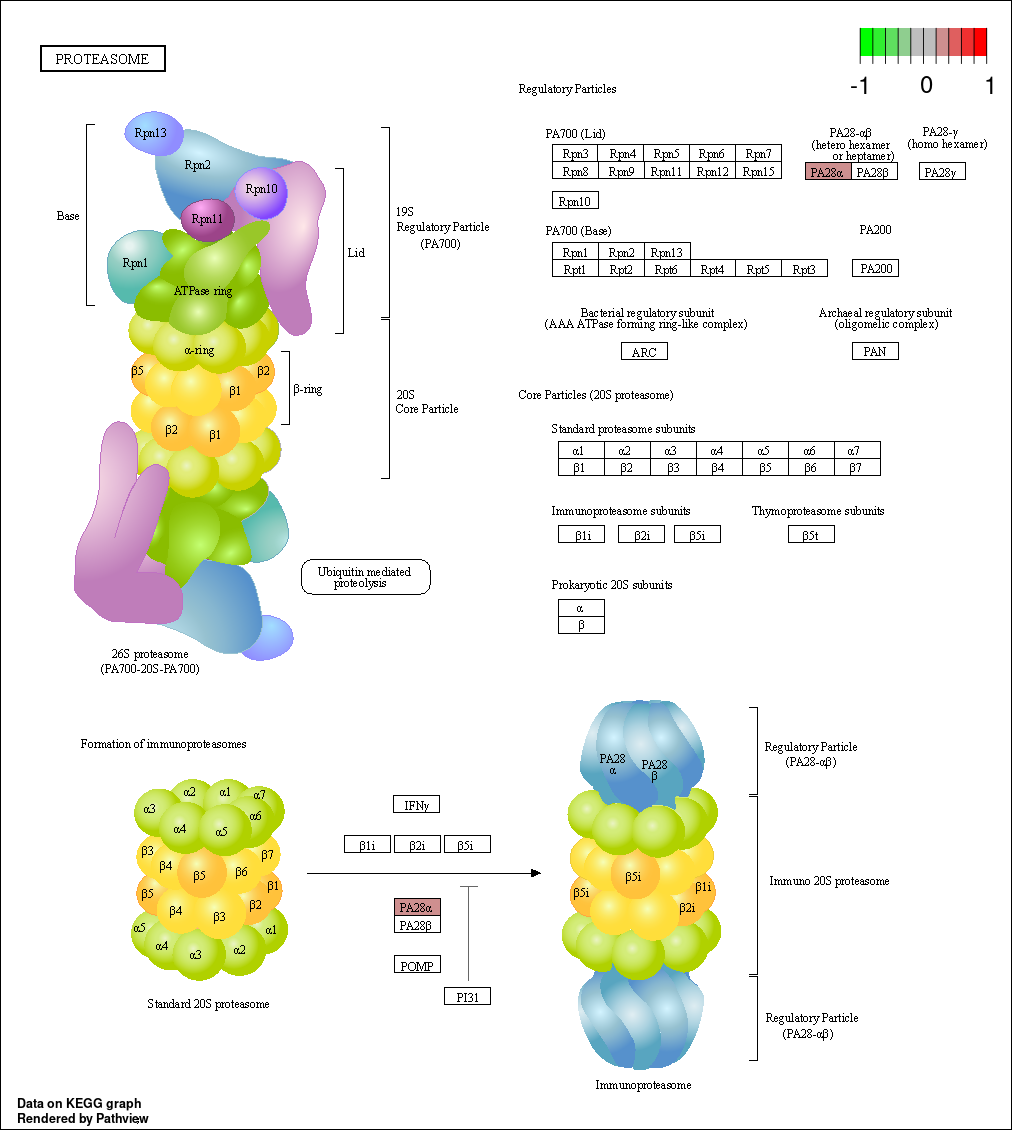
\includegraphics[width=13.56in]{thesis_fig/hsa03050.pathview} \caption{通路'Proteasome'(ID:hsa03050)}\label{fig:keggPath}
\makeatletter \egroup

\bgroup \def\@captype{figure}
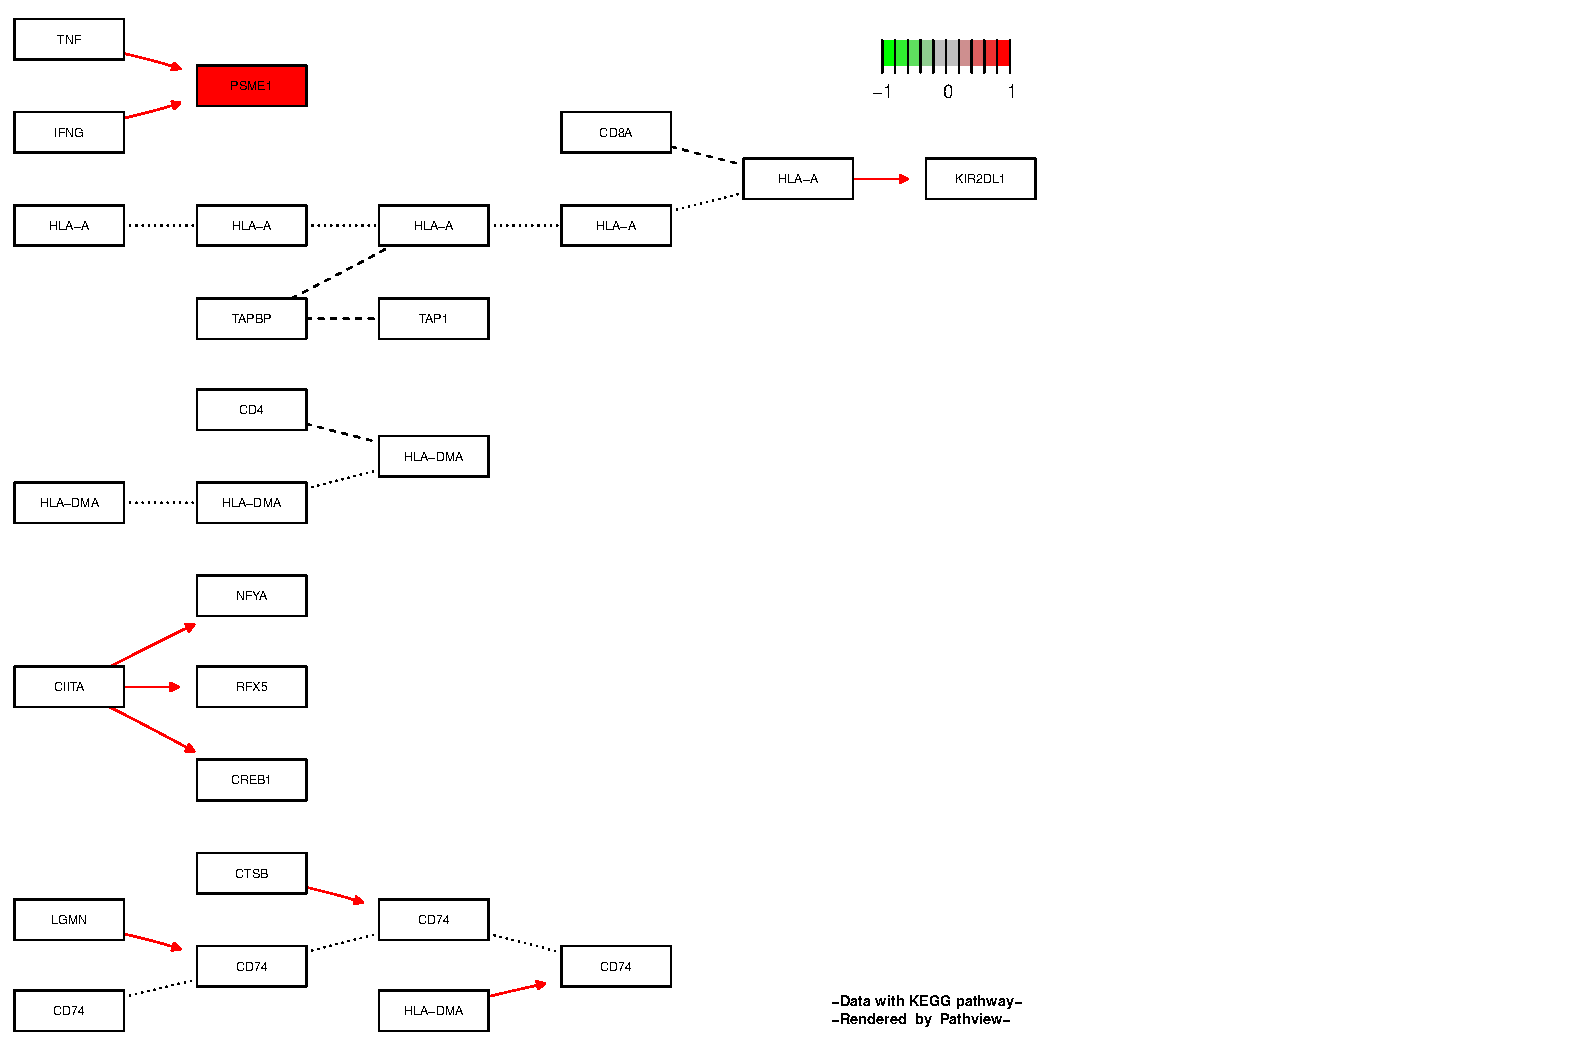
\includegraphics[width=14.88in]{thesis_fig/hsa04612.pathview} \caption{通路'Antigen processing and presentation'(ID:hsa04612)}\label{fig:fig10}
\makeatletter \egroup

\hypertarget{ux7ed3ux8bbaux4e0eux4e34ux5e8aux8f6cux5316}{%
\subsubsection{结论与临床转化}\label{ux7ed3ux8bbaux4e0eux4e34ux5e8aux8f6cux5316}}

本次分析目的为探究类风湿性关节炎单核细胞衍生巨噬细胞的促炎症和代谢功能。巨噬细胞的激活和极化在炎症发展的前馈和反馈机制中起到了重要作用\textsuperscript{\protect\hyperlink{ref-hu_regulation_2008}{4}},了解其极化后功能的改变对治疗类风湿性关节炎具有启发意义。本次分析结果表明,相比于极化健康巨噬细胞(M2, IL-4处理组),类风湿关节炎单核细胞衍生的巨噬细胞(M1, LPC + IFN处理组)具有显著高表达的'PA28'基因(entrezid: 5720,见Tab. \ref{tab:topAnno}),富集于'Antigen processing and presentation'和'Proteasome'通路(Tab. \ref{tab:richRes})。'PA28'基因可能成为治疗类风湿关节炎的临床用药靶点。

\hypertarget{githubux6570ux636e}{%
\subsection{Github数据}\label{githubux6570ux636e}}

本次研究涉及的所有数据和脚本已上传至:
\url{https://github.com/Cao-lab-zcmu/metabo_stat/tree/master/lixiao}。

\hypertarget{ux9644ux64cdux4f5cux622aux56fe}{%
\subsection{附:操作截图}\label{ux9644ux64cdux4f5cux622aux56fe}}

\bgroup \def\@captype{figure}
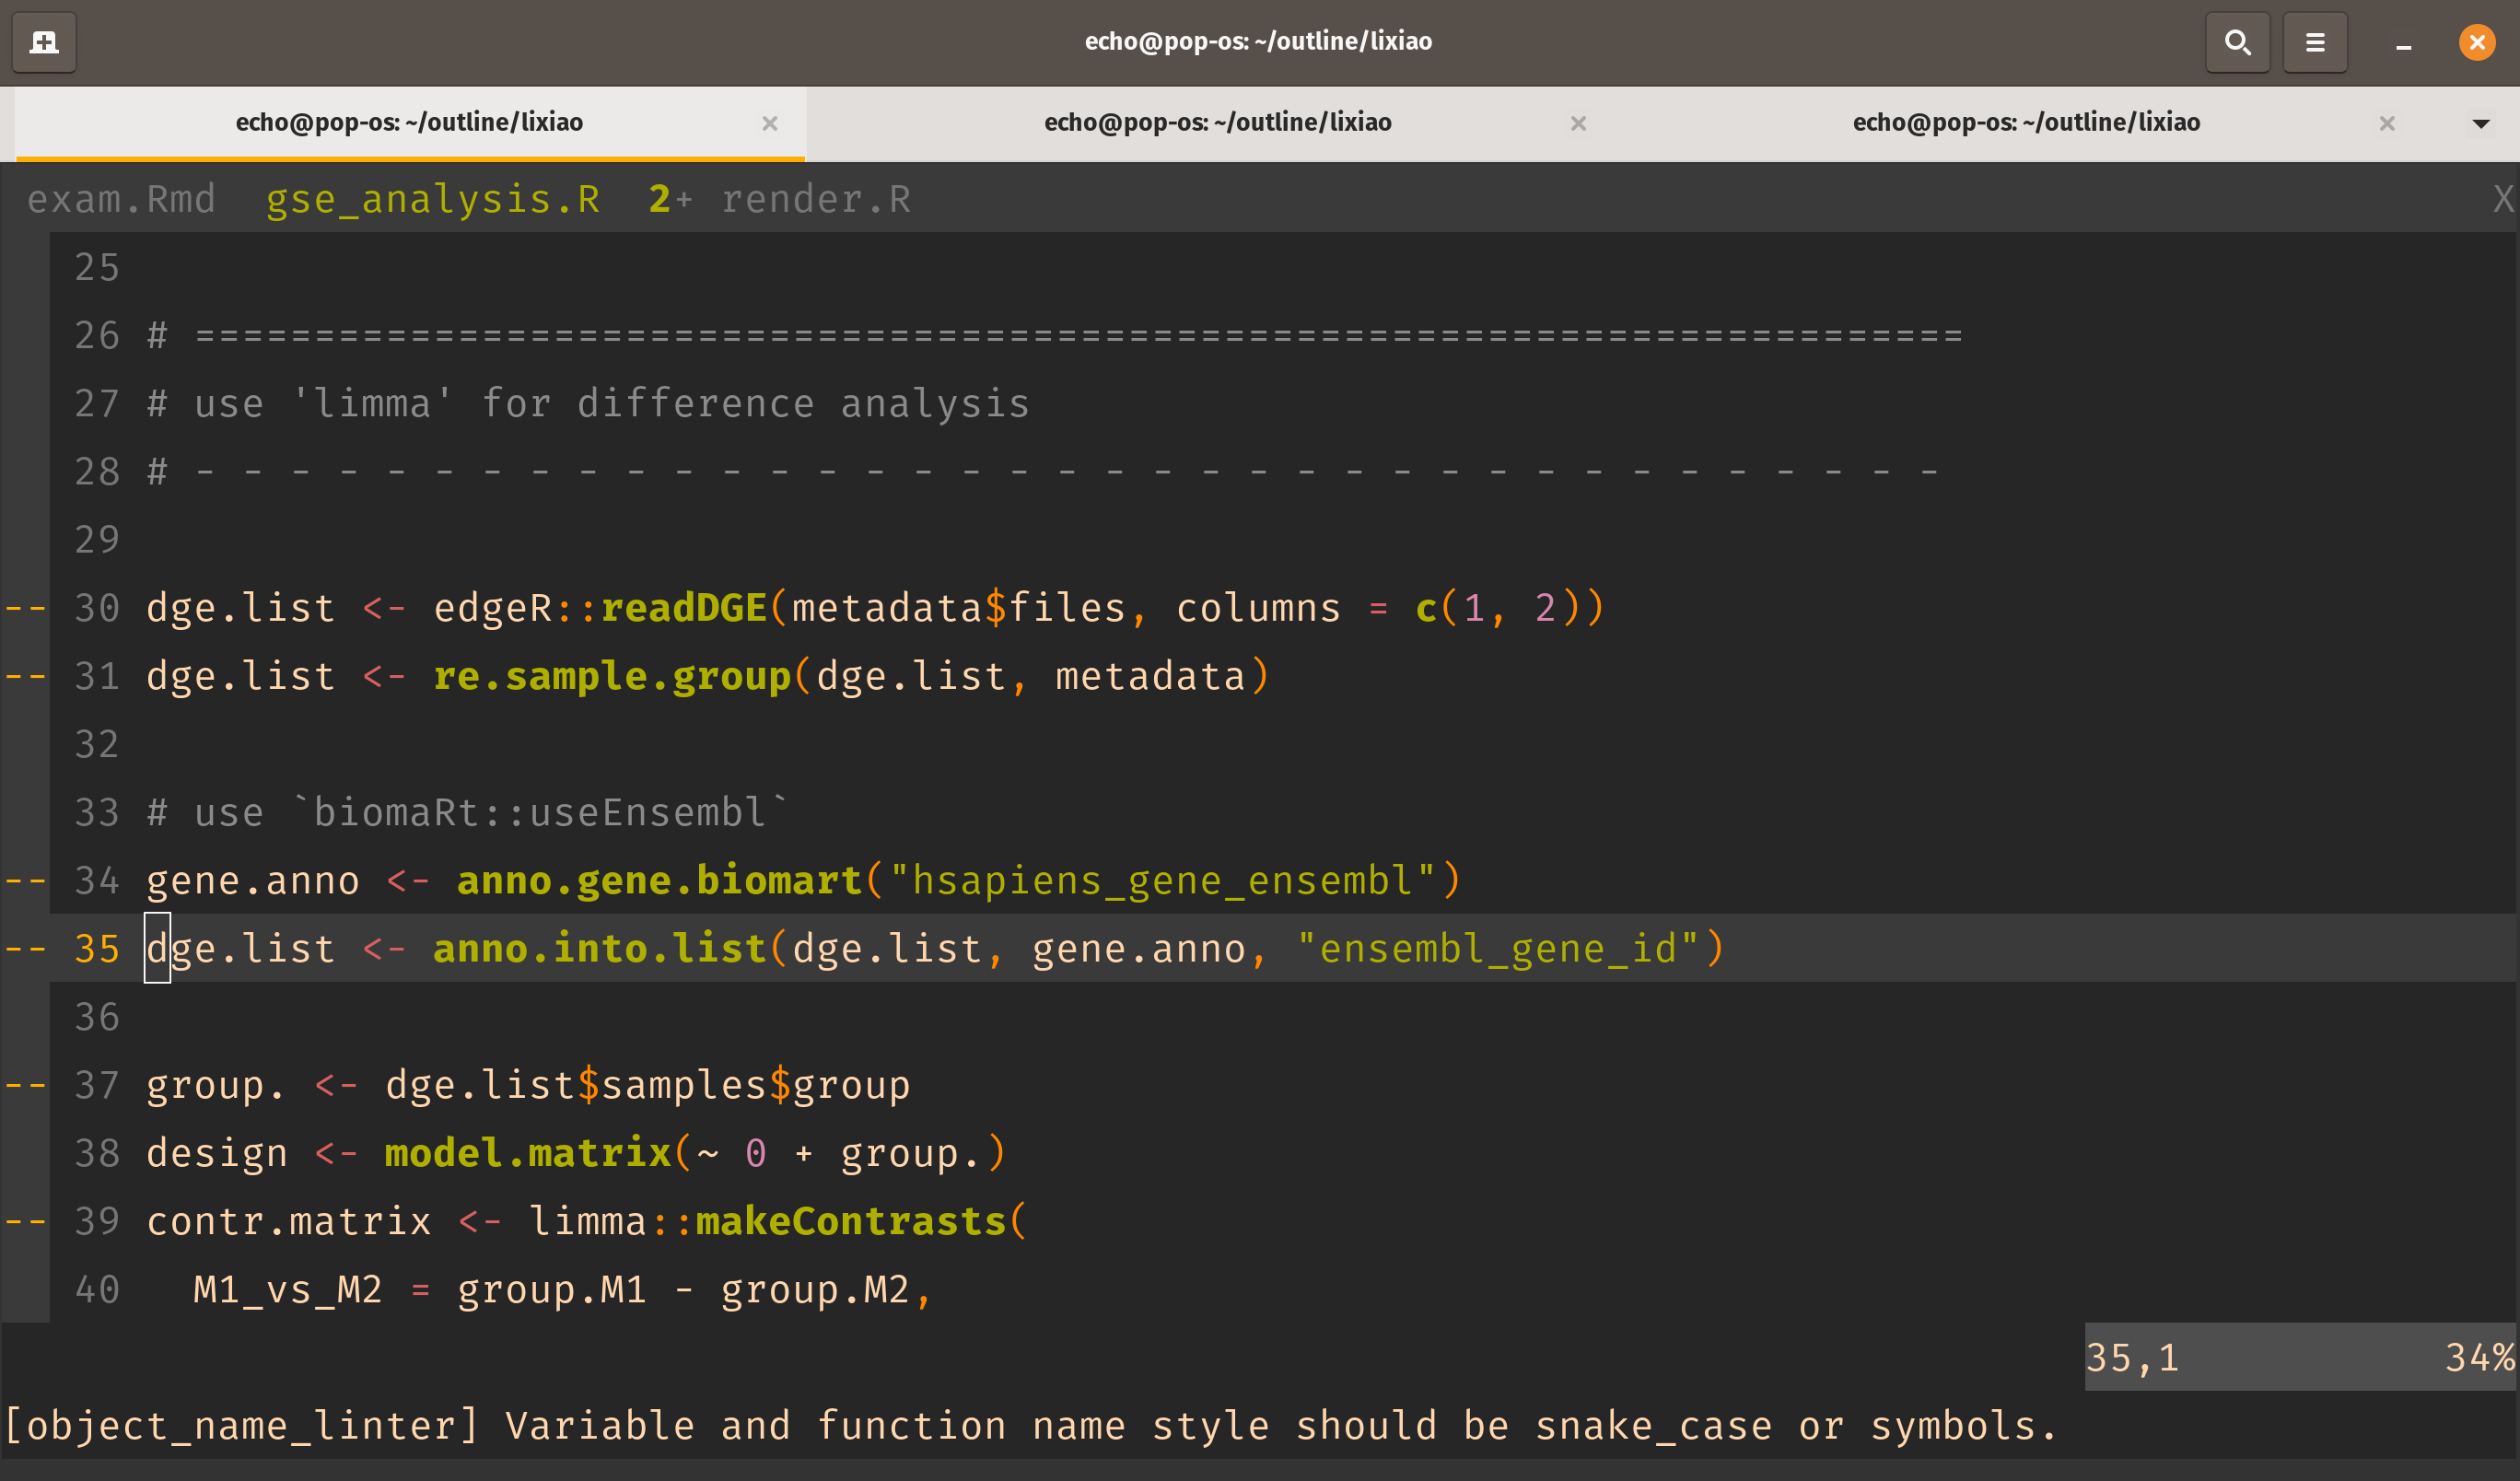
\includegraphics[width=13.89in]{thesis_fig/writeScript_capture} \caption{编写分析脚本(VIM界面)}\label{fig:fig12}
\makeatletter \egroup

\bgroup \def\@captype{figure}
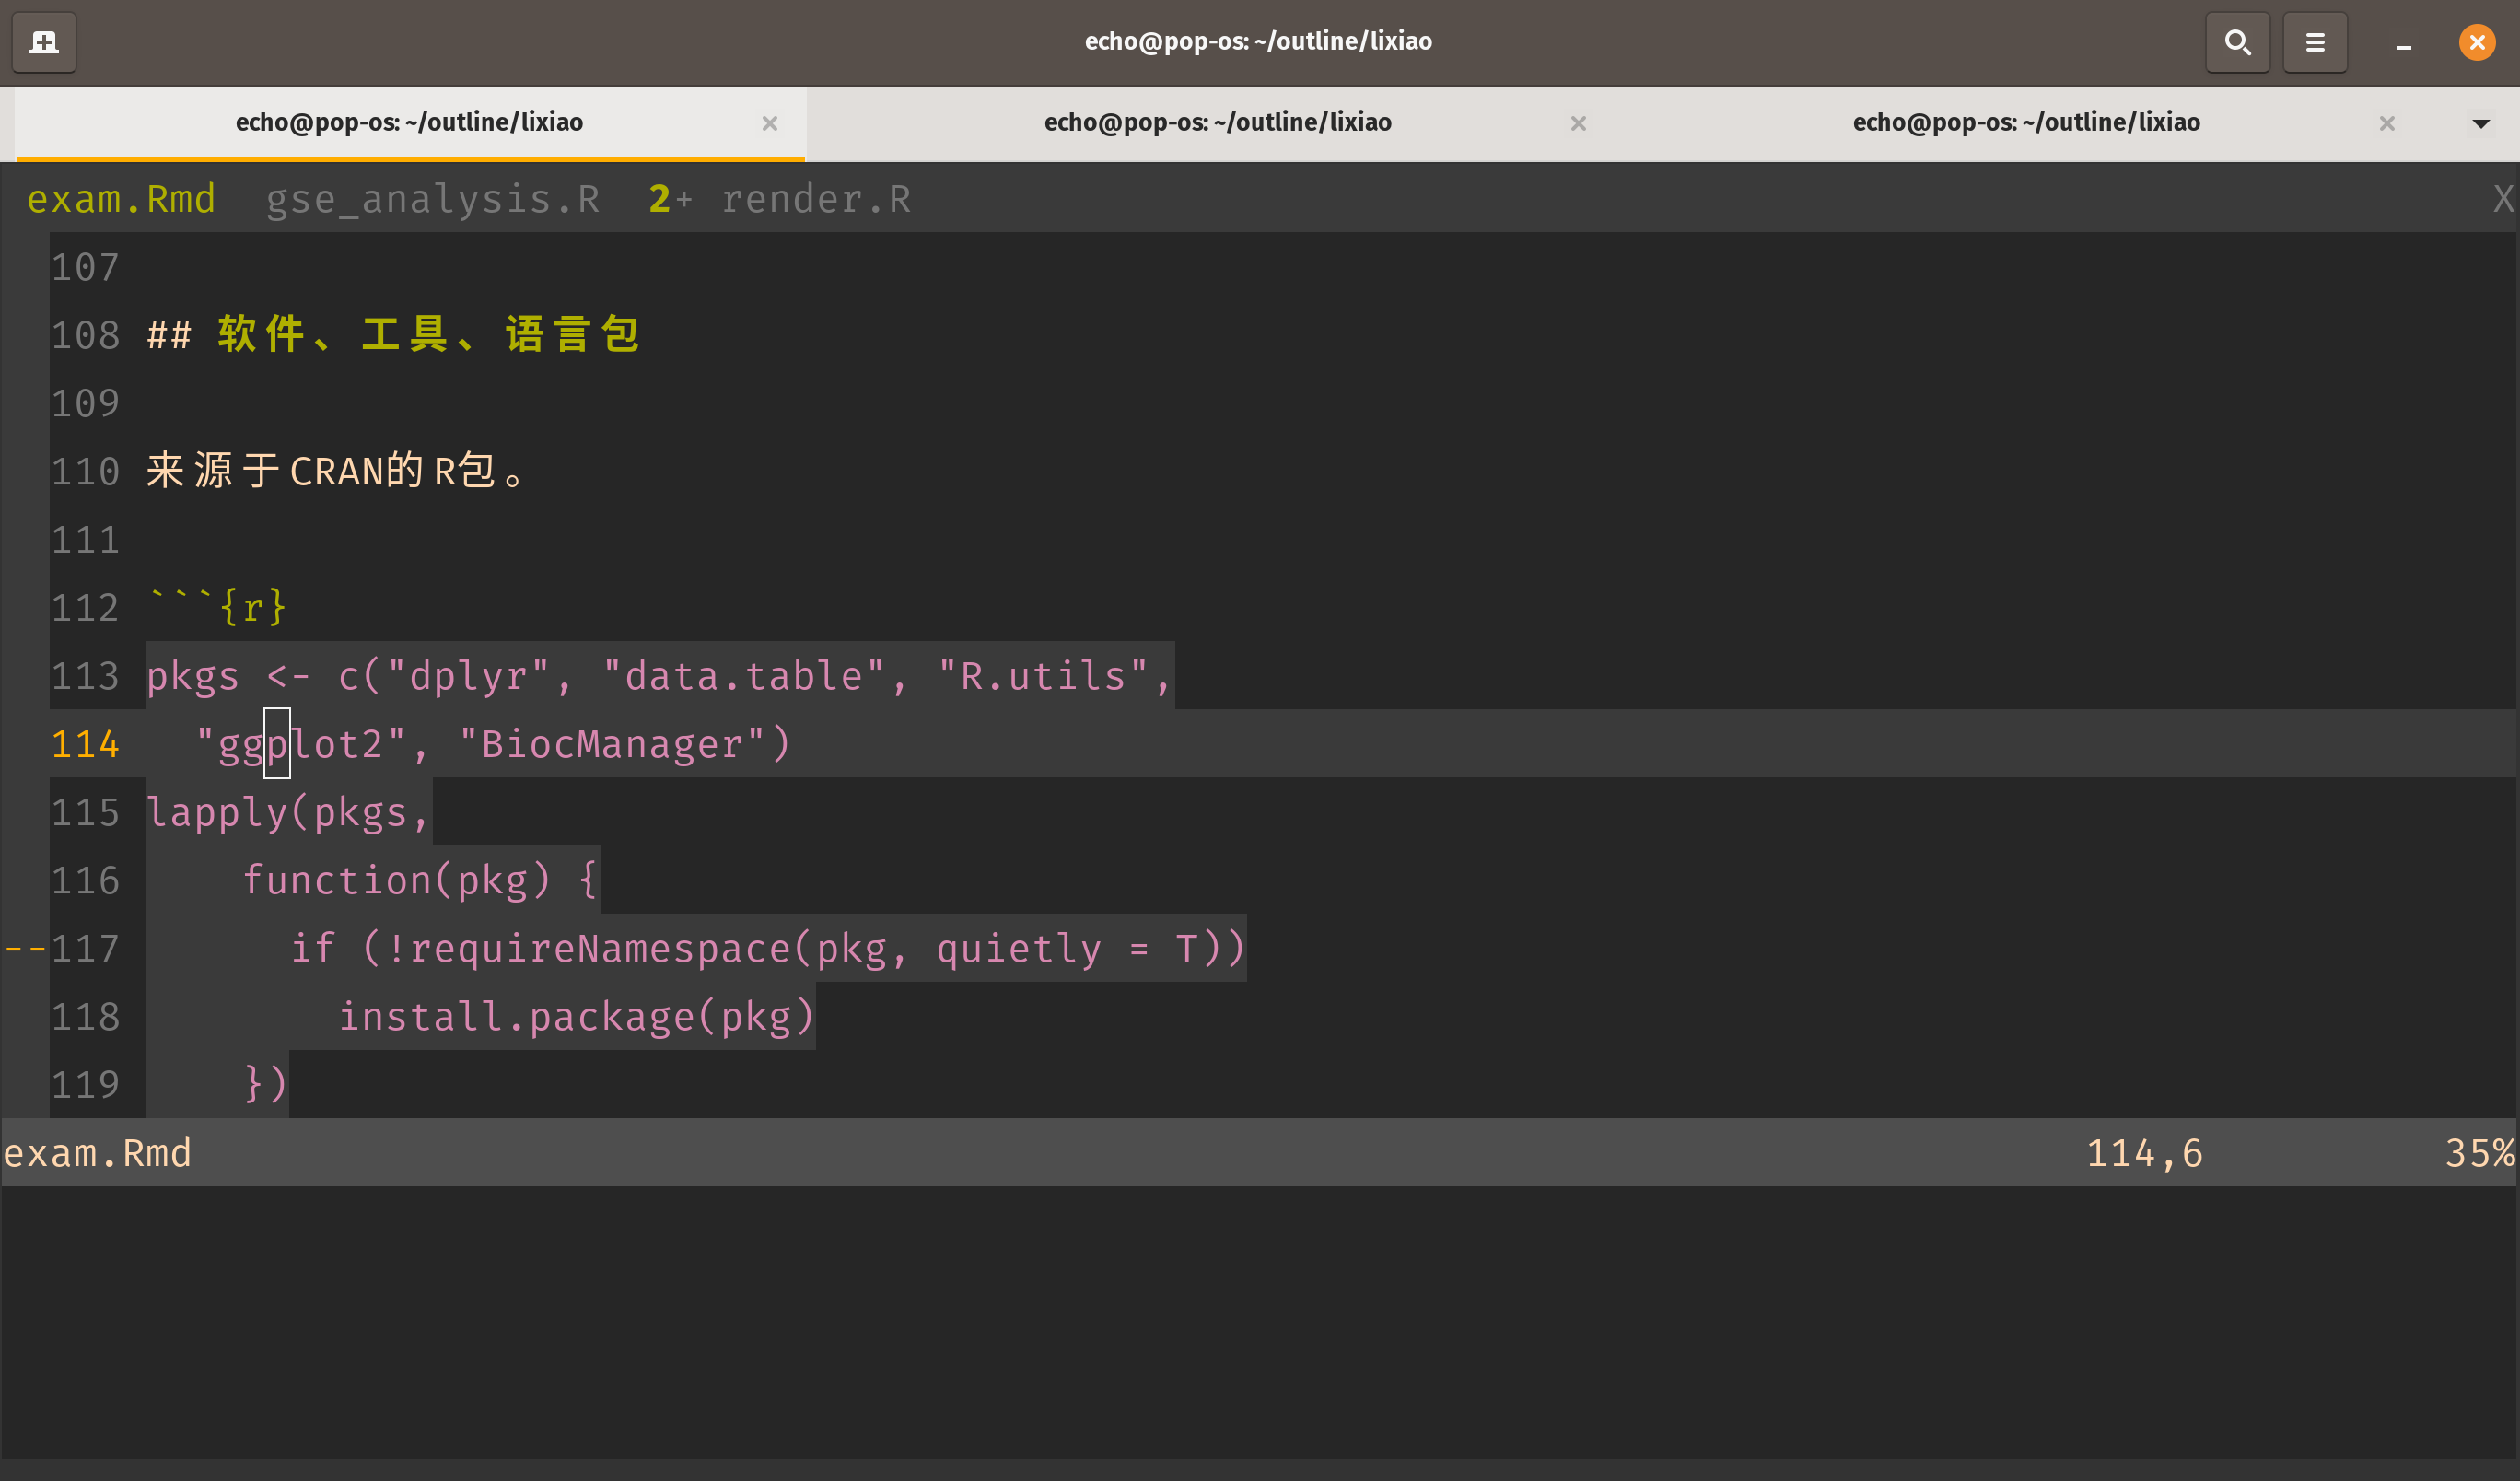
\includegraphics[width=13.89in]{thesis_fig/writeReport_capture} \caption{编写分析报告}\label{fig:fig13}
\makeatletter \egroup

\bgroup \def\@captype{figure}
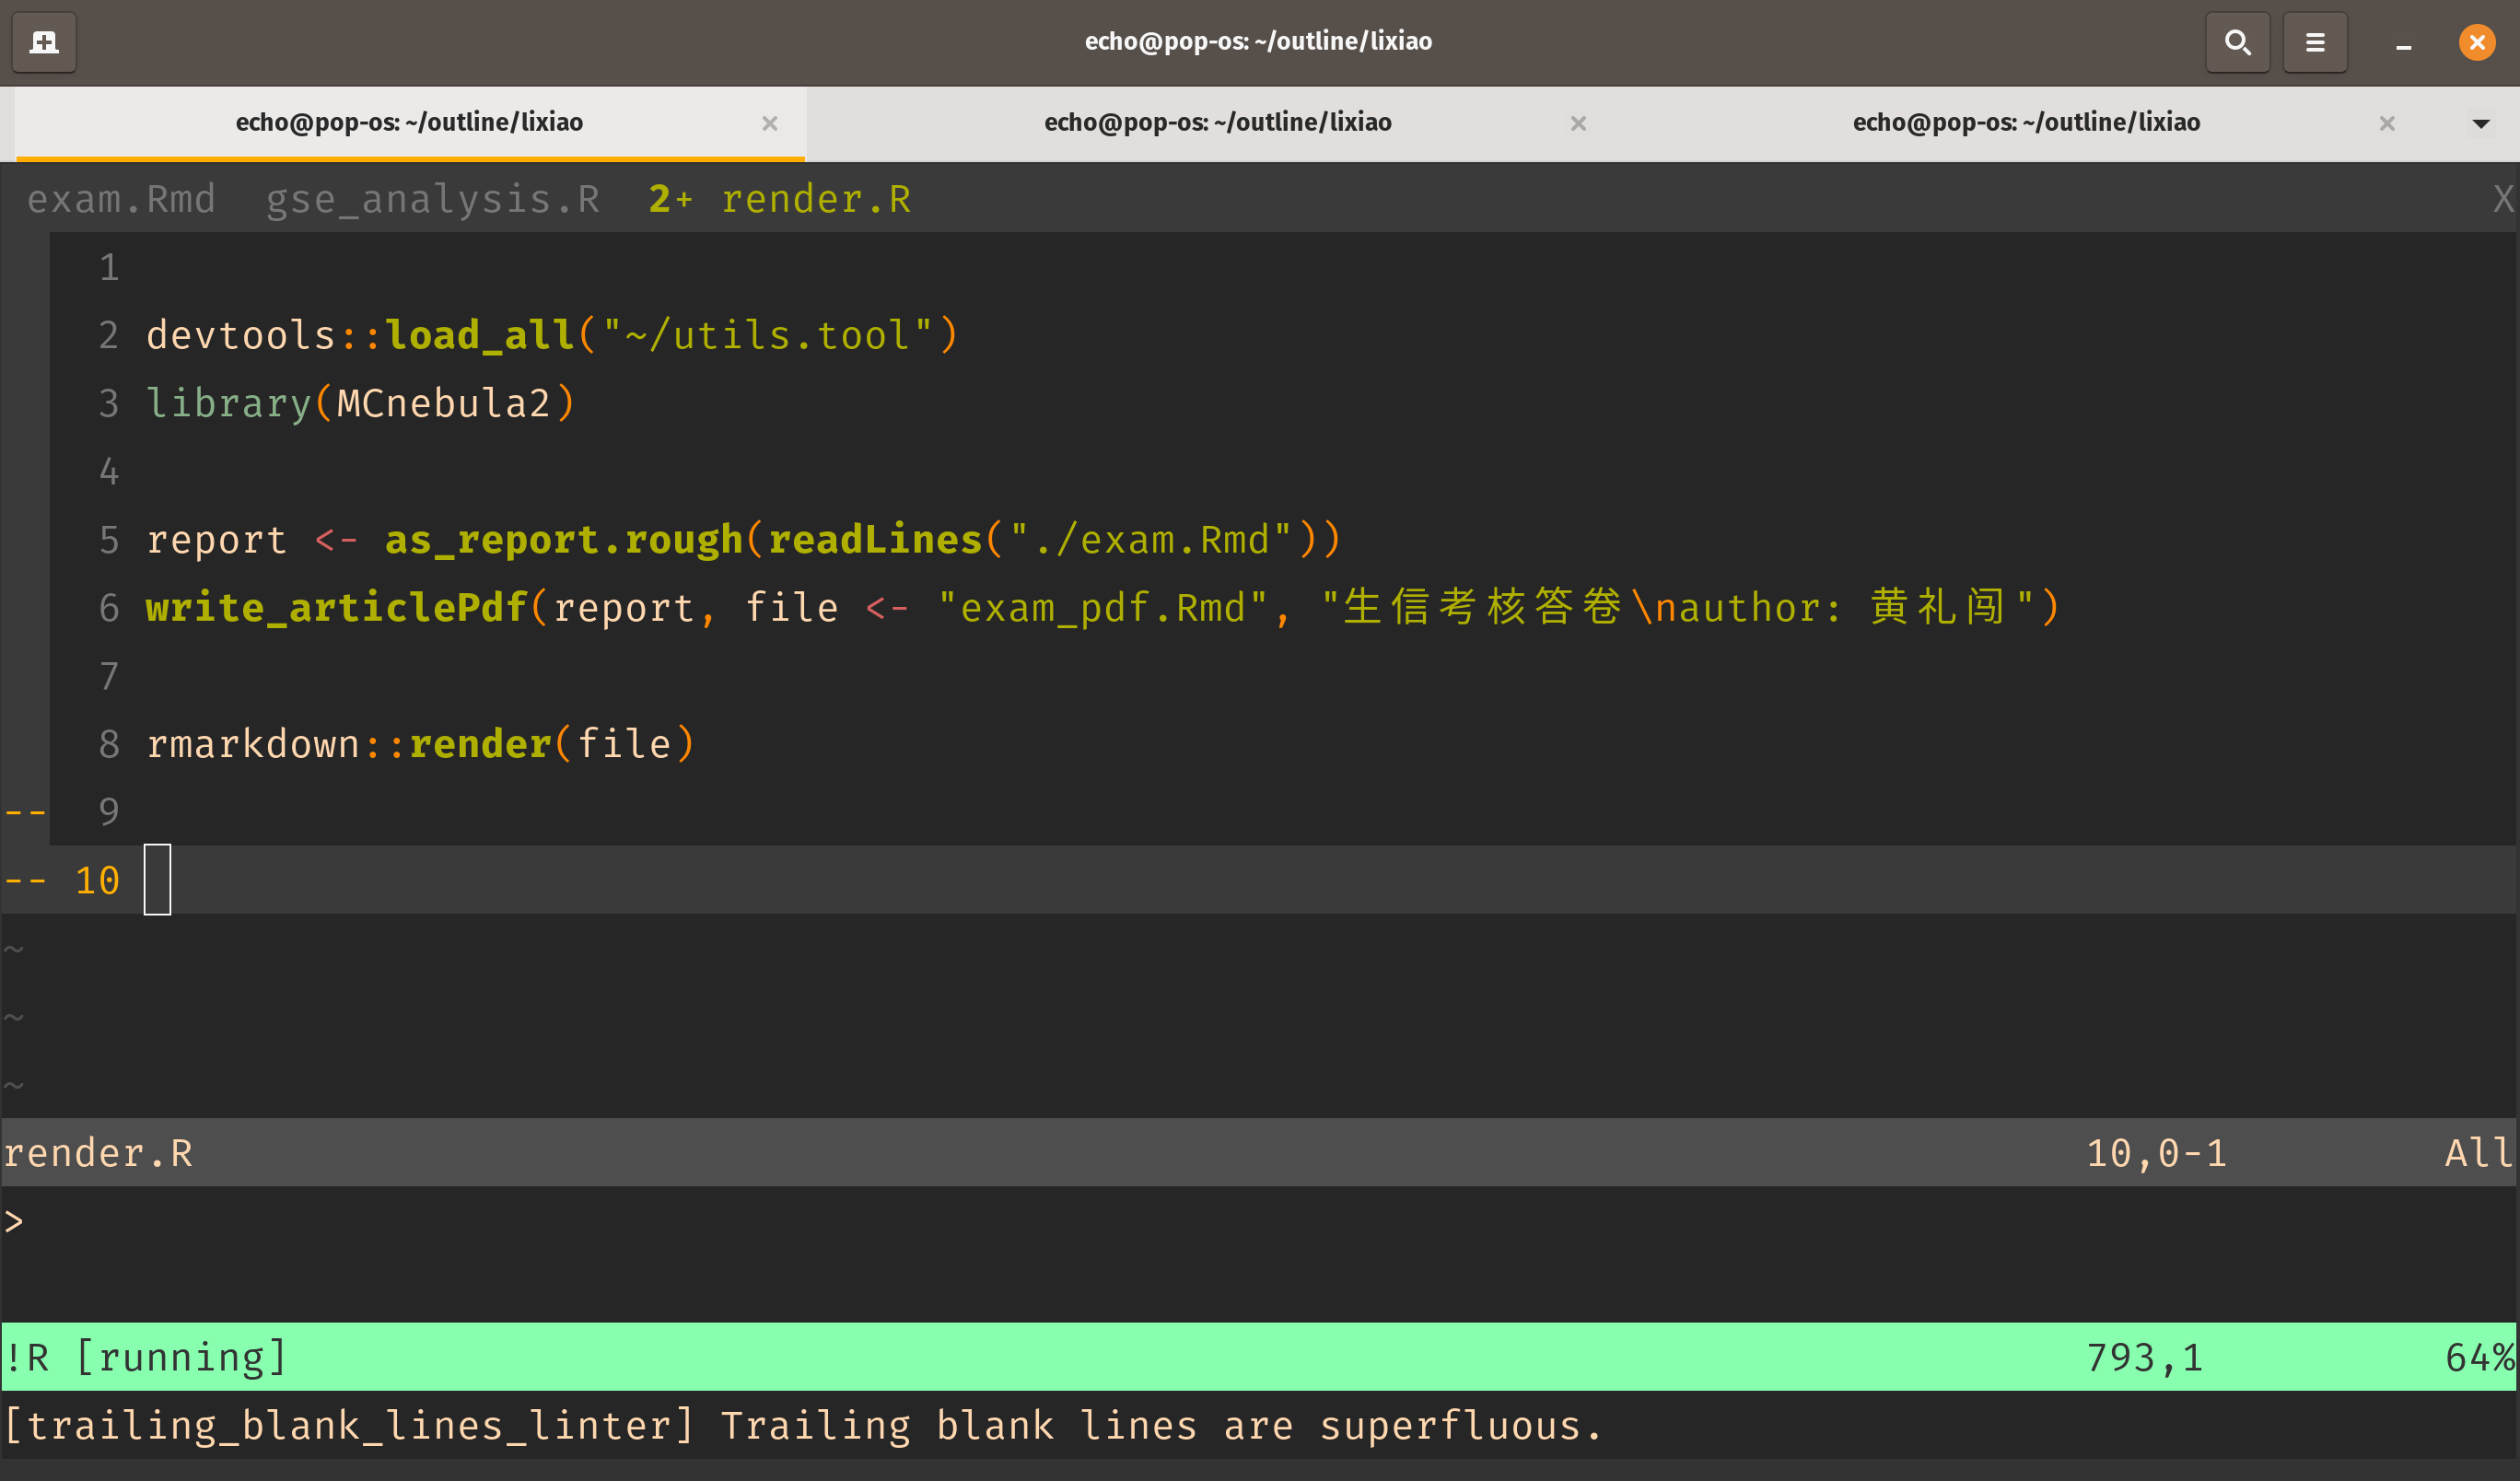
\includegraphics[width=13.89in]{thesis_fig/outputReport_capture} \caption{输出分析报告为PDF格式}\label{fig:fig14}
\makeatletter \egroup

\bgroup \def\@captype{figure}
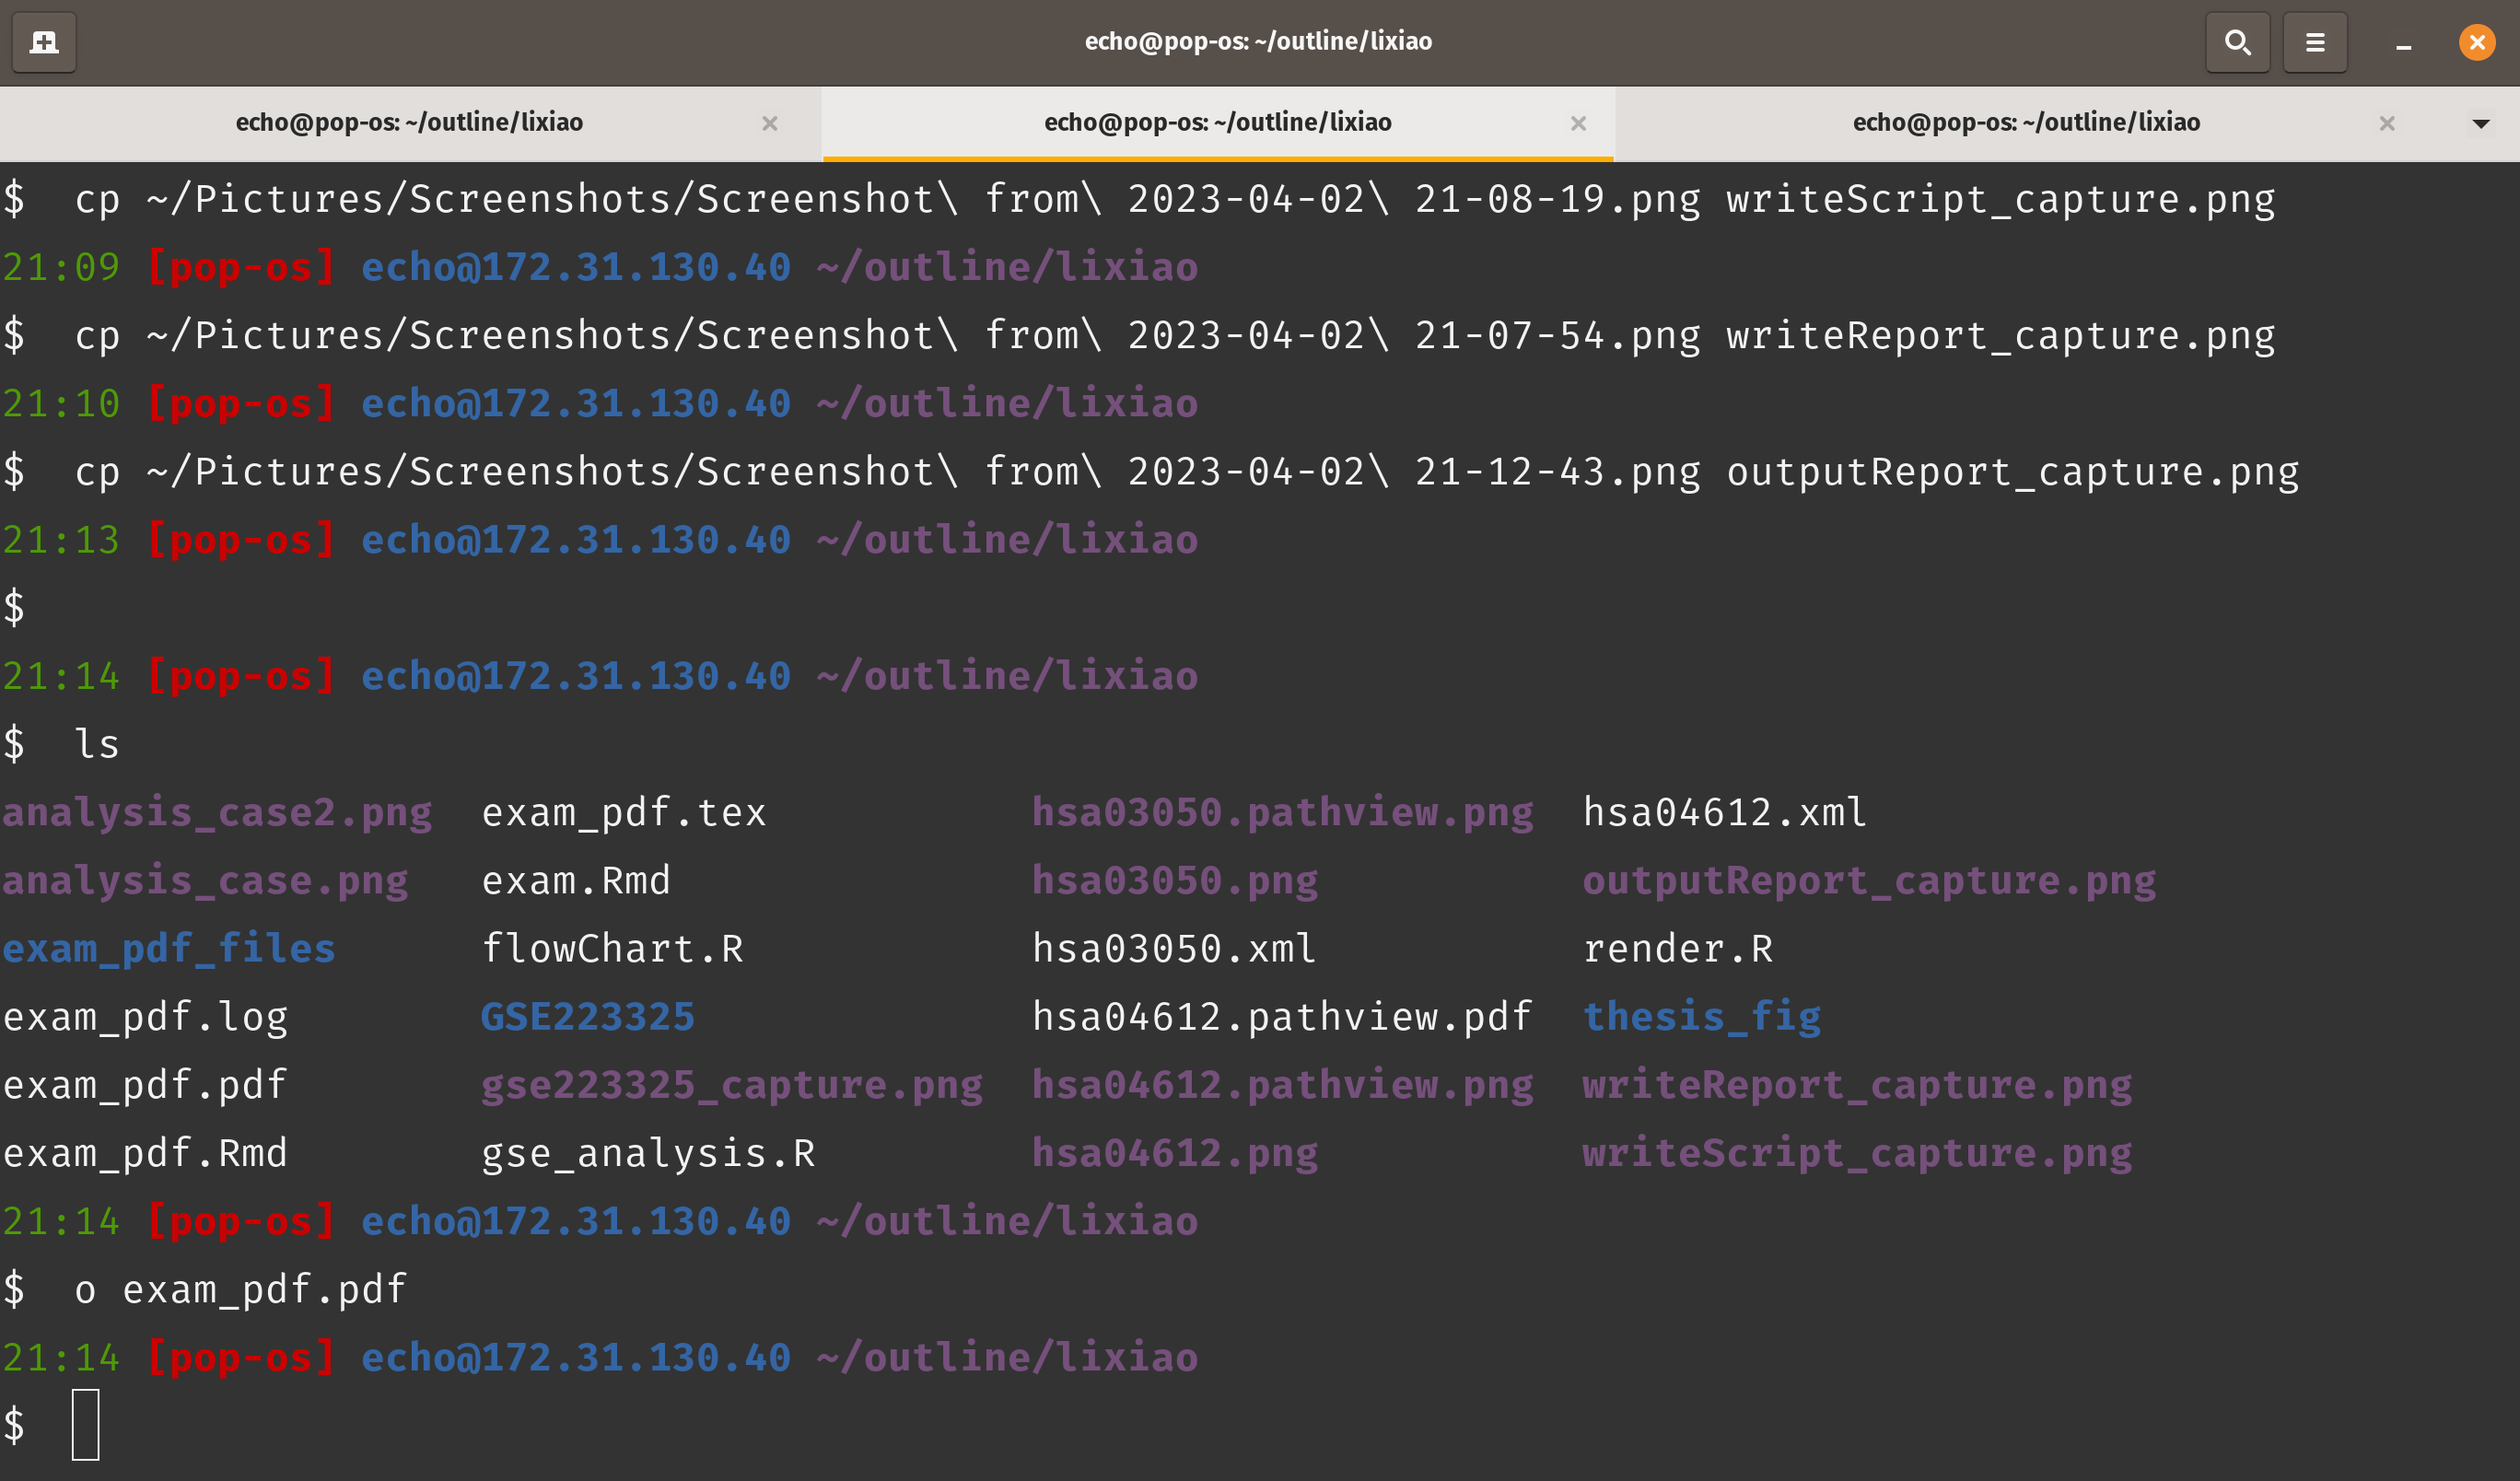
\includegraphics[width=13.89in]{thesis_fig/workDir_capture} \caption{工作目录}\label{fig:fig15}
\makeatletter \egroup

\bgroup \def\@captype{figure}
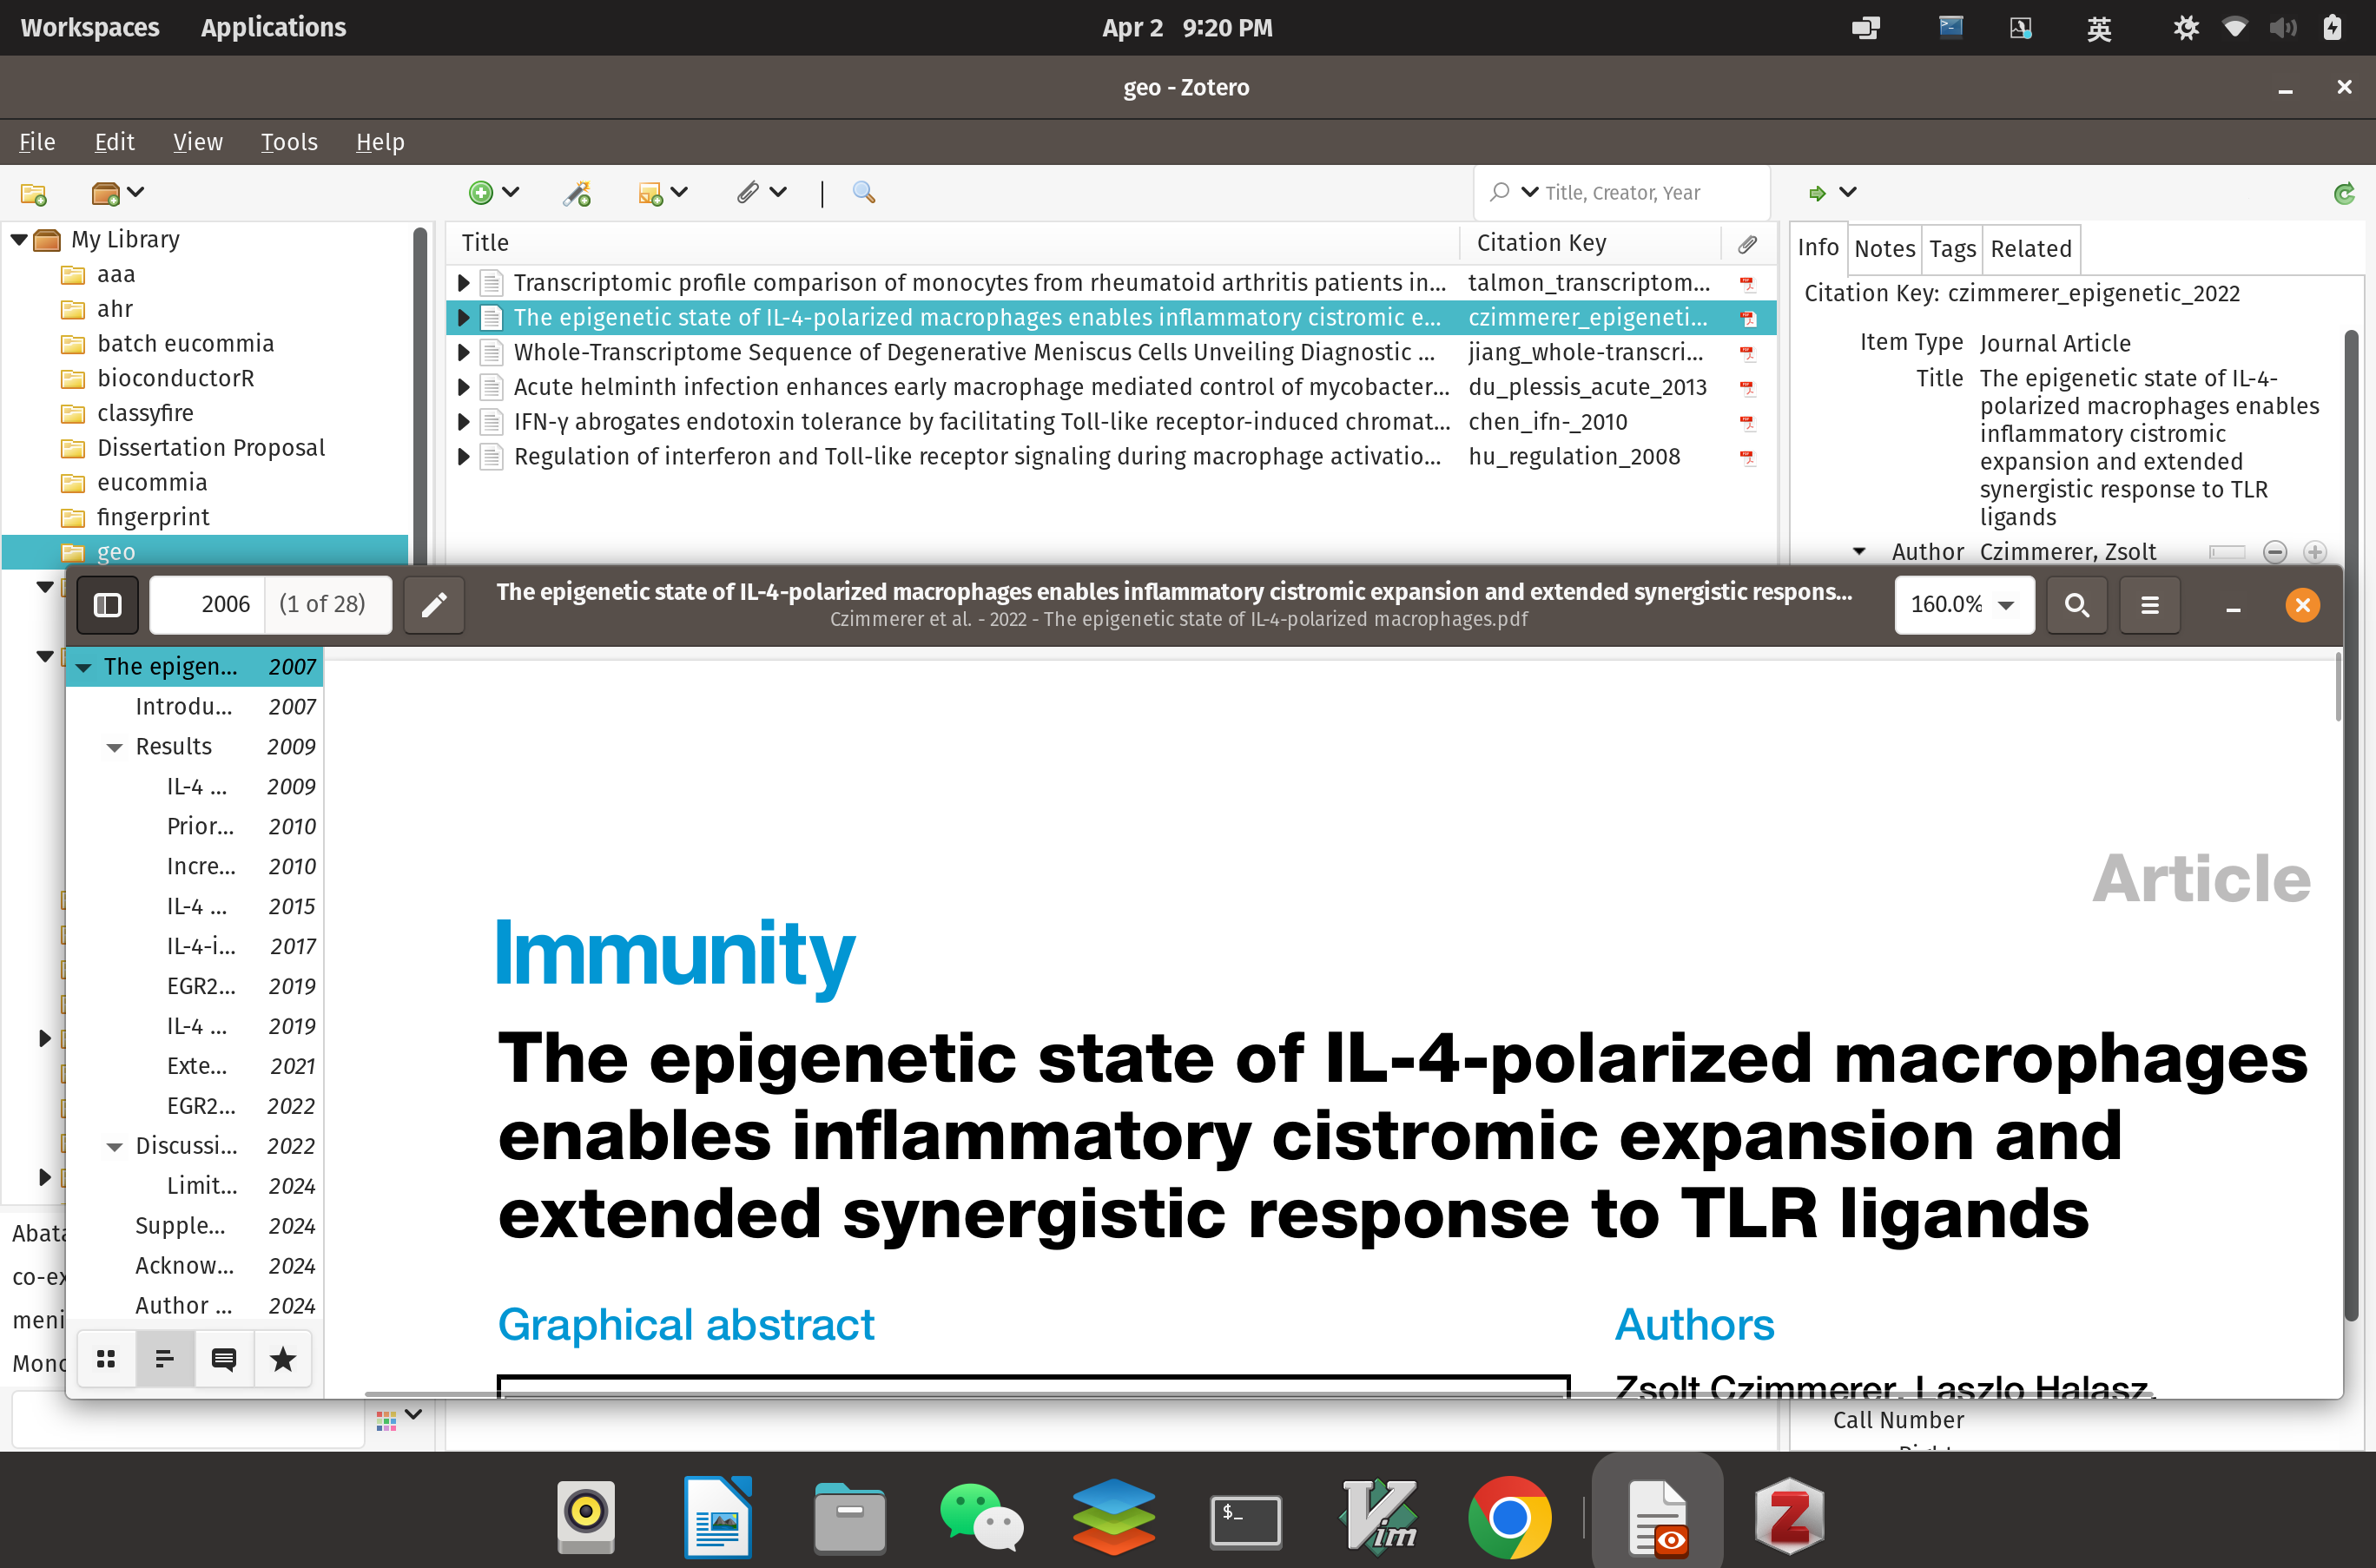
\includegraphics[width=13.89in]{thesis_fig/manageRef} \caption{查阅和管理文献}\label{fig:fig16}
\makeatletter \egroup

\hypertarget{bibliography}{%
\section*{Reference}\label{bibliography}}
\addcontentsline{toc}{section}{Reference}

\hypertarget{refs}{}
\begin{CSLReferences}{0}{0}
\leavevmode\vadjust pre{\hypertarget{ref-sadik_il4i1_2020}{}}%
\CSLLeftMargin{1. }%
\CSLRightInline{Sadik, A. \emph{et al.} \href{https://doi.org/10.1016/j.cell.2020.07.038}{{IL4I1 Is} a {Metabolic Immune Checkpoint} that {Activates} the {AHR} and {Promotes Tumor Progression}}. \emph{Cell} \textbf{182}, 1252--1270.e34 (2020).}

\leavevmode\vadjust pre{\hypertarget{ref-2020s}{}}%
\CSLLeftMargin{2. }%
\CSLRightInline{Wozniak, J. M. \emph{et al.} \href{https://doi.org/10.1016/j.cell.2020.07.040}{Mortality {Risk Profiling} of {Staphylococcus} aureus {Bacteremia} by {Multi-omic Serum Analysis Reveals Early Predictive} and {Pathogenic Signatures}}. \emph{Cell} \textbf{182}, 1311--1327.e14 (2020).}

\leavevmode\vadjust pre{\hypertarget{ref-czimmerer_epigenetic_2022}{}}%
\CSLLeftMargin{3. }%
\CSLRightInline{Czimmerer, Z. \emph{et al.} \href{https://doi.org/10.1016/j.immuni.2022.10.004}{The epigenetic state of {IL-4-polarized} macrophages enables inflammatory cistromic expansion and extended synergistic response to {TLR} ligands}. \emph{Immunity} \textbf{55}, 2006--2026.e6 (2022).}

\leavevmode\vadjust pre{\hypertarget{ref-hu_regulation_2008}{}}%
\CSLLeftMargin{4. }%
\CSLRightInline{Hu, X., Chakravarty, S. D. \& Ivashkiv, L. B. \href{https://doi.org/10.1111/j.1600-065X.2008.00707.x}{Regulation of interferon and {Toll-like} receptor signaling during macrophage activation by opposing feedforward and feedback inhibition mechanisms}. \emph{Immunological Reviews} \textbf{226}, 41--56 (2008).}

\leavevmode\vadjust pre{\hypertarget{ref-chen_ifn-_2010}{}}%
\CSLLeftMargin{5. }%
\CSLRightInline{Chen, J. \& Ivashkiv, L. B. \href{https://doi.org/10.1073/pnas.1007816107}{{IFN-\(\gamma\)} abrogates endotoxin tolerance by facilitating {Toll-like} receptor-induced chromatin remodeling}. \emph{Proceedings of the National Academy of Sciences} \textbf{107}, 19438--19443 (2010).}

\leavevmode\vadjust pre{\hypertarget{ref-law_guide_2020}{}}%
\CSLLeftMargin{6. }%
\CSLRightInline{Law, C. W. \emph{et al.} \href{https://doi.org/10.12688/f1000research.27893.1}{A guide to creating design matrices for gene expression experiments}. \emph{F1000Research} \textbf{9}, 1444 (2020).}

\end{CSLReferences}

\end{document}
